\documentclass[autoref,10pt]{disser}
\usepackage{pscyr}
\usepackage{cite}
\usepackage{psfrag}
\usepackage{color}
%\usepackage[colorlinks,bookmarksopen]{hyperref}
\usepackage[warn]{mathtext}
\usepackage[english,russian]{babel}
\usepackage{cite}
\usepackage{amsmath,amssymb}
%\usepackage{booktabs}
\usepackage{array,hhline,longtable}
\renewcommand{\rmdefault}{ftm}
\usepackage[utf8]{inputenc}
\usepackage{graphicx}
\usepackage{indentfirst}
\usepackage{wrapfig}
\DeclareSymbolFont{T2Aletters}{T2A}{cmr}{m}{it}
\everymath{\displaystyle}
\singlespacing

\usepackage[
a5paper, includefoot,
left=1.5cm, right=1.5cm, top=1.5cm, bottom=1.8cm,
headsep=0cm, footskip=1.3cm
]{geometry}

\newcommand{\dbl}{\hbox to 9pt {/\hss /} }
\newcounter{enumv}
\newcounter{enumvi}
\renewcommand{\theenumv}{\arabic{enumv}}
\renewcommand{\theenumvi}{\arabic{enumvi}*}

\newenvironment{theotherbib1}[1][.]
{\begin{list}{\theenumv#1\hspace{5pt}}{
\begin{center}\bf\large Литература \end{center}
\usecounter{enumv}
\topsep=0pt\labelsep=2pt\itemsep=0pt\itemindent=\parindent
\listparindent=-\parindent}}
{\end{list}}



\newenvironment{theotherbib2}[1][.]
{\begin{noindlist}{\theenumvi#1\hspace{5pt}}{
\begin{center}\bf\large Литература \end{center}
\usecounter{enumvi}
\topsep=0pt\leftmargin=15pt\labelsep=2pt\itemsep=0pt\
\listparindent=-10pt}}
{\end{noindlist}}



\makeatletter

\renewcommand{\@makefntext}[1]{\parindent=1em\noindent
              \hbox to 1.8em{\hss$^{\@thefnmark)}$}#1}
\renewcommand{\@makefnmark}{\hbox{\mathsurround=0pt$^{\@thefnmark)}$}}
\renewcommand{\@biblabel}[1]{#1.\hfill}
\renewcommand{\@pnumwidth}{1.7em}
\newcommand{\l@bib}[2]{\hbox to\textwidth{{\bf #1}
 \leaders\hbox to .8em{\hss.\hss}\hfill \makebox[\@pnumwidth][r]{\bf #2}}\par}
\makeatother

\newenvironment{mylist}[1][.]%
{\begin{list}{\arabic{enumi}#1\hspace{5pt}}{\usecounter{enumi}%
\topsep=0pt\labelwidth=0pt\leftmargin=0pt\labelsep=0pt\itemsep=0pt\parsep=0pt%
\listparindent=6pt\itemindent=0pt}}%
{\end{list}}



\renewcommand{\sectionfont}{\noindent\normalsize\bfseries} % Номер главы полужирным
\renewcommand{\subsectionfont}{\noindent\normalsize\bfseries}
\renewcommand{\subsubsectionfont}{\noindent\normalsize\bfseries}
\renewcommand{\appendixfont}{\normalsize\bfseries}

\renewcommand{\sectionindent}{0cm}
\renewcommand{\subsectionindent}{0cm}

\renewcommand{\aftersection}{6pt plus .1pt}
\renewcommand{\beforesection}{12pt plus .1pt}
\renewcommand{\aftersubsection}{3pt plus .1pt}
\setcounter{tocdepth}{2}
\setcounter{page}{1}
\setlength{\parskip}{1.0pt} 
\setlength{\parindent}{0.6cm}

\begin{document}
\Russian
\thispagestyle{empty}
\vspace{1.5cm}
\centerline{Российская академия наук}
\centerline{Институт прикладной физики}
\vspace{3cm}
\centerline{А В Т О Р Ы}
\vspace{0.8cm}
\begin{center}
\large 
\textbf{ПАРАМЕТРИЧЕСКАЯ ГЕНЕРАЦИЯ НИЗКОЧАСТОТНЫХ ВОЛН ЭЛЕКТРОНАМИ УСКОРЕННЫМИ В УСЛОВИЯХ ЭЛЕКТРОННО-ЦИКЛОТРОННОГО РЕЗОНАНСА}
\end{center}
\vspace{2cm}
\centerline{\large Препринт № }
\vfill
\centerline{Нижний Новгород}
\centerline{2011}
\newpage
\thispagestyle{empty}
\begin{flushleft}
УДК
\end{flushleft}


Экспериментально исследован эффект генерации потоков ускоренных частиц в условиях электронного циклотронного резонанса (ЭЦР) в ближнем поле антенн, при этом в плазме наблюдается диамагнитный эффект: уменьшение индукции внешнего магнитного поля в области, содержащие быстрые частицы. Показано, что при амплитудной модуляции ВЧ сигнала, подводимого к излучающей антенне, в плазме возбуждаются электромагнитные волны на частоте моуляции. Предложено использовать данный эффект в качестве  инструмента параметрической генерации  низкочастотных волн в замагниченной плазме при проведении соответствующих активных экспериментов в ионосфере Земли. 

\newpage
\section{Введение}
Низкочастотные волны, возбуждаемые в диапазонах ультранизких, крайне низких и очень низких частот (УНЧ , КНЧ и ОНЧ), представляют значительный интерес с точки зрения организации сверхдальней радиосвязи, пассивной и активной волновой диагностики параметров ионосферы и магнитосферы Земли, а также рассматриваются как инструмент активного воздействия на околоземную плазму, например --- с целью организации высыпаний энергичных частиц радиационных поясов. Для решения указанных задач актуальным является поиск эффективных методов генерации низкочастотных волн в плазме ближнего космоса. 
При проведении активных экспериментов в околоземной плазме одной из важнейших задач является генерация свистовых волн ($\sqrt{f_{ci}f_{ce}}<F<f_{ce}\ll f_{pe}$, где $F$ --- частота НЧ излучения, $f_{ce}, f_{ci}, f_{pe}$ --- электронная циклотронная, ионная циклотронная и плазменная частоты, соответственно), играющих ключевую роль в динамике магнитосферы, и являющихся удобным средством мониторинга плазменного  окружения Земли. 

Эффективность традиционных методик возбуждения свистовых волн с использованием компактных спутниковых антенных систем невелика вследствие больших длин волн излучения.  Использование наземных СДВ-станций сопряжено с  серьезными финансовыми расходами для поддержания их функциональности, обусловленными, в основном,  большой общей длиной используемых антенн (до 80 км) [Siple].
Один из путей повышения эффективности генерации низкочастотных волн состоит в создании протяженных излучающих токовых систем непосредственно  в околоземной плазме. Для этих целей ранее предлагалось использовать модулированные пучки заряженых частиц, инжектируемые с борта космических аппаратов [4], либо нелинейные эффекты в поле интенсивных волн с относительно высокими частотами, возбуждаемых спутниковыми и наземными передатчиами [5, 6]. В частности, методики возбуждения ОНЧ волн в ионосфере, используемые в наземных нагревных стендах, основаны на эффекте модуляции проводимости нижних слоев ионосферы под действием ВЧ поля, модулированного на низкой частоте, что ведет к формированию источника ОНЧ излучения непосредственно в ионосфере.

В данной работе  предлагается использовать параметрический метод генерации волн свистового диапазона с использованием традиционных антенных систем, размещаемых на КА. Описываемая в работе методика основана  на  нелинейных эффектах, развивающихся в плазме, окружающей антенные системы, под действием мощной ВЧ ($P\sim100$\,Вт) накачки  при приближении рабочей частоты $f$ к "главным" резонансным частотам: электронной плазменной $f_{pe}$, электронной циклотронной $f_{ce}$ и их гармоникам. В резонансных условиях возможны возбуждение высокодобротных колебаний в плазме и антенных цепях~\ref{WHISPER}, нагрев плазмы и генерация потоков ускоренных заряженных частиц~\ref{Pulinets,Galperin,Huang}.
В качестве основного механизма генерации предлагается использовать эффект резонансного ускорения электронов под воздействием ВЧ импульса накачки в условиях электронного-циклотронного резонанса, т.е при приближении рабочей частоты бортового передатчика к значениям локальной электронной циклотронной частоты и ее гармоник.  Этот механизм представляется наиболее перспективным и надежным, так как, в отличие от других плазменных резонансов, не связан с  коллективными явлениями в плазме и представлет собой надежно воспроизводимый, эффект. 

Если ВЧ сигнал, подводимый к антенне, модулирован по амплитуде с частотой $f_{m}$, то поток ускоренных электронов, и, соответственно, наведенный в возмущенной области плазмы магнитный момент изменяются с периодом модуляции. В результате, протяженная область пространства, в которую из ближней зоны передатчика поступает модулированный поток ускоренных по поперечной энергии электронов, может выступать в роли "бестелесной" антенны, излучающей волны на частоте модуляции в окружающую плазму. Эффективную длина такой антенны в типичных условиях ионосферы может достигать значений до нескольких километров, что превышает длину традиционных антенн КА, и, тем самым, повышает эффективность возбуждения свистовых волн в целом. Широкополосная перестройка по низкой частоте производится изменением частоты модуляции $f_{m}$. Следует также отметить, что полученная таким образом ``бестелесная'' антенна --- магнитного типа, что повышает эффективность возбуждения электромагнитных волн.

Целью работы является экспериментальное исследование диамагнитного эффекта и оценка возможности генерации квазистационарных магнитных полей и ОНЧ волн при ЭЦР нагреве лабораторной плазмы моделями бортовых антенн КА. Модельные лабораторные эксперименты были проведены на крупномасштабном плазменном стенде "Крот". Результаты работы могут быть использованы при планировании соответствующих экспериментов в ионосфере Земли.
Предлагаемая в настоящей работе схема возбуждения ОНЧ волн может оказаться эффективнее, чем описанный  в~\ref{Gushchin} параметрический механизм возбуждения НЧ свистовых волн ВЧ волновыми пучками, основанный на генерации дрейфовых электронных токов под действием усредненной пондеромоторной силы, при реализации в активных ионосферных экспериментах. 

%Большие наземные станции, всилу своего стационарного базирования, являются локальными исследовательскими инструментами, оперирующими только с одной магнитной силовой трубкой, соответствующей географическому расположению  стенда. С этой точки зрения, альтернативу составляет возбуждение НЧ волн с борта космических аппаратов (КА), которые, по мере своего движения по орбите, пересекают  области ионосферы, соответствующие различным широтам, долготам и локальному времени суток и, тем самым, являются инструментами оперативной диагностики и воздействия на параметры околоземной плазмы в целом. Однако, одним из недостатков такой методики является низкая эффективность прямого возбуждения волн ОНЧ диапазона бортовыми антеннами КА, обусловленная, в первую очередь, их малыми размерами по сравнению с длинами волн ОНЧ диапазона; характерные размеры применяемых антенн не превышают значений $L\sim10\div{}100$~м. Прямое возбуждение ОНЧ волн такими антеннами малоэффективно, так как они являются электрическим малыми для волн данного диапазона ($\lambda/L\gg{}1$). Ограничение на максимальный размер бортовых антенн связано с ограничением на максимальную взлетную массу спутника и сложностью развертывания антенной системы на орбите. Повышение мощности передатчиков космического базирования также сопряжено с серьезными трудностями.
%
% Ниже кратко рассмотрены результаты соответствующих космических экспериментов.
%
%
%
%
%
%
%

%\section{Модельные лабораторные эксперименты} 
\section{Описание эксперимента}
Экспериментальный стенд ``Крот'' (\mbox{рис.\ref{fig:KROT}}) создан в ИПФ РАН для моделирования физических процессов в плазме ионосферы и магнитосферы Земли. Установка представляет собой вакуумную камеру, изготовленную из немагнитной нержавеющей стали, диаметром $3$\,м и длиной $10$\,м.  Давление остаточного газа в камере не превышает  $p = 5\cdot10^{-6}$ торр. 
Магнитное поле пробочной конфигурации создается с помощью соленоида, установленного внутри вакуумного объема. Длительность импульса тока в соленоиде составляет $20$ мс, что существенно больше времен исследуемых плазменных процессов. Величина поля $B_{0}$ в минимуме может составлять до $1$ кГс.
Квазиоднородный цилиндрический столб замагниченной плазмы длинной около $500$\,см и диаметром $150$\,см формировался в результате импульсного индукционного разряда; для создания плазмы используются два ВЧ-генератора с частотой $5$ МГц и выходной мощностью до $1$ МВт в импульсе длительностью $1.5$ мс.

Непрерывный напуск газа рабочего газа (аргона) осуществляется через пьезокерамический натекатель. Установка работает в импульсно-периодическом режиме с частотой повторения $0.05$---$0.2$ Гц. Максимальная плотность плазмы в момент пробоя достигает $n_{0} \approx 10^{13}$ см$^{-3}$, после окончания работы генераторов плазма распадается с характерным временем порядка нескольких миллисекунд, зависящим от величины магнитного поля $B_{0}$. Распад определяется процессом амбиполярной диффузии вдоль магнитного поля. На стадии распада плазмы устанавливается квазистационарная температура электронов $T_{e} \approx 0.2$ --- $1$\,эВ, в зависимости от выбранной мощности ВЧ генераторов. Ионная температура не превышает $T_{i} \sim 1$\,эВ. Эксперименты, в которых были получены результаты, представляемые в работе, выполнялись в режиме распадающейся плазмы.
\begin{figure}[H]
    \centering
    \includegraphics*[width=0.9\columnwidth]{pics/KROT.eps}
    \caption{Схема экспериментальной установки ``Крот''; цифрами на схеме обозначены:  $(1)$ рабочая камера,  $(2)$ система напуска рабочего газа, $(3)$  соленоиды для создания внешнего магнитного поля, $(4)$ плазмосоздающие индукторы, $(5)$ двойной зонд, $(6)$ антенна накачки, $(7)$ двойной электрический зонд, $(8)$ зонд с СВЧ резонатором, $(9)$ магнитный зонд, $(10)$ двухкоординатная позиционная система; также представлена цилиндрическая система  координат, используемая при описании результатов.}
    \label{fig:KROT}
 \end{figure}

Принципиальная схема включения радиотехничекой аппаратуры в ходе  экспериментов представлена на \mbox{рис.~\ref{fig:scheme_setup}}. Мощный ВЧ сигнал ($f=65\div{}85$\,МГц, $P\simeq300$\,Вт) подводился к рамочной антенне диаметром $7$\,см, установленной на оси плазменного столба ($r=0$\,см), в форме импульса длительностью $\tau=0.1\div1000$\,мкс. В ВЧ генераторе был предусмотрен режим глубокой (до $100\%$) амплитудной модуляции сигнала на низкой частоте, $f_m=0.1\div{}10$\,МГц. 
\begin{figure}[H]
    \centering
    \includegraphics*[width=0.7\columnwidth]{pics/scheme_setup.eps}
    \caption{Принципиальная схема включения радиотехнической аппаратуры в ходе проведенных в работе экспериментов.}
    \label{fig:scheme_setup}
 \end{figure}


Регистрация возбуждаемых в плазме квазистационарных и НЧ магнитных полей осуществлялась шестивитковыми магнитными зондами диаметром~$1.8$\,см, помещенными в электростатические экраны и изолированными от плазмы тонким слоем диэлектрика. 

Для диагностики плотности плазмы в широком интервале значений использовались зонды с СВЧ-резонатором на отрезке двухпроводной линии~\ref{Stenzel,Yanin}. Температура электронов измерялась двойным электрическим зондом~\ref{UHF_probe}. 
%\begin{figure}[H]
%    \centering
%    \includegraphics*[width=0.8\textwidth]{scheme_setup}
%    \caption{Схема модельных экспериментов по параметрическому возбуждению НЧ волн в плазме потоками ускоренных электронов, формируемых в условиях ЭЦР.}
%    \label{fig:scheme_setup}
%\end{figure}

При выборе параметров лабораторного эксперимента использовались преобразования подобия~\ref{Alfven}, позволяющие напрямую связать результаты космических и лабораторных экспериментов через масштабный множитель $\gamma$. В случае лабораторного моделирования активных ионосферных экспериментов в качестве множителя $\gamma$ естественно выбрать отношение характерных размеров бортовой антенны $L$ и ее уменьшенной лабораторной модели $l$: $\gamma{}=L/l$. 

В модельном лабораторном эксперименте удалось сохранить бесстолкновительный режим взаимодействия плазмы с ближним полем передатчика, характерный для ионосферных экспериментов (т.е. $l_{ei}/L\gg{}1$, $l_{ei}$---длина свободного пробега электронов, обусловленная кулоновскими столкновениями), что позволило провести качественное моделирование по немасштабируемому параметру $\nu_{ei}$ --- частоте электрон-ионных кулоновских столкновений.

Параметры экспериментов, приведенны в \mbox{таб.~\ref{tab:value_scaling_ionosphere}}.
\begin{table}[H]
{
   \hfill{}
   \small
   \centering %центрируем таблицу
   \begin{tabular}{|m{3cm}|m{2.3cm}|m{4.5cm}|}
     \hline
     \textbf{Параметр} & \textbf{Ионосфера} & \textbf{Лабораторная плазма}\\\hline
     Концентрация электронов $n_{e}$,\,см$^{-3}$ & $10^{3}\div{}10^{6}$ & $10^{7}\div{}10^{10}$ ($10^{6}\div{}10^{11}$)\\\hline
     Температура электронов $T_{e}$,\,эВ & $0.2\div5$ & $0.2\div5$ ($0.3\div3$)\\\hline
     Индукция статического магнитного поля $B$,\,Гс & $0.2\div0.5$ & $20\div50$ ($10\div100$)\\\hline
     Размер антенны $L$,\,см & $1000$ & $10$ ($7$)\\\hline
     Частота $f$,\,МГц &$0.1\div10$& $10\div{}1000$ ($65\div 80$)\\\hline
     Мощность передатчика $P$,\,Вт &$100\div1000$& $100\div1000$ ($300$)\\\hline
   \end{tabular}
   \hfill{}
}
\caption{Параметры активных ионосферных и модельных лабораторных экспериментов при значении масштабного множителя $\gamma = 100$; в скобках приведены фактические параметры эксперимента на стенде ``Крот''.}
   \label{tab:value_scaling_ionosphere}
\end{table}
\section{Экспериментальные результаты}
\subsection{Возмущения магнитного поля, формируемые одиночным радиоимпульсом}
Как показали эксперименты, в плазме уверенно регистрируется диамагнитный эффект, обусловленный резонансным ускорением электронов в ближней зоне антенны. На \mbox{рис.\ref{fig:pump}} показаны типичные осциллограммы импульса накачки (\mbox{рис.\ref{fig:pump}}a), подаваемого на антенну в условиях ЭЦР, неинтегрированного сигнала с магнитного зонда (\mbox{рис.\ref{fig:pump}}b),  когда он находится напротив витков рамочной антенны  и соответствующего возмущения $\Delta{}B$ магнитного поля $B_{0}$ (\mbox{рис.\ref{fig:pump}}с). Величина диамагнитного эффекта в ходе экспериментов составляла $\Delta{}B\sim{}10^{-2}$\,Гс.

\begin{figure}[H]
  \centering
  \def\svgwidth{0.6\columnwidth} % sets the image width, this is optional
  %% Creator: Inkscape inkscape 0.48.0, www.inkscape.org
%% PDF/EPS/PS + LaTeX output extension by Johan Engelen, 2010
%% Accompanies image file 'pulse_demo.ps' (pdf, eps, ps)
%%
%% To include the image in your LaTeX document, write
%%   \input{<filename>.pdf_tex}
%%  instead of
%%   \includegraphics{<filename>.pdf}
%% To scale the image, write
%%   \def\svgwidth{<desired width>}
%%   \input{<filename>.pdf_tex}
%%  instead of
%%   \includegraphics[width=<desired width>]{<filename>.pdf}
%%
%% Images with a different path to the parent latex file can
%% be accessed with the `import' package (which may need to be
%% installed) using
%%   \usepackage{import}
%% in the preamble, and then including the image with
%%   \import{<path to file>}{<filename>.pdf_tex}
%% Alternatively, one can specify
%%   \graphicspath{{<path to file>/}}
%% 
%% For more information, please see info/svg-inkscape on CTAN:
%%   http://tug.ctan.org/tex-archive/info/svg-inkscape

\begingroup
  \makeatletter
  \providecommand\color[2][]{%
    \errmessage{(Inkscape) Color is used for the text in Inkscape, but the package 'color.sty' is not loaded}
    \renewcommand\color[2][]{}%
  }
  \providecommand\transparent[1]{%
    \errmessage{(Inkscape) Transparency is used (non-zero) for the text in Inkscape, but the package 'transparent.sty' is not loaded}
    \renewcommand\transparent[1]{}%
  }
  \providecommand\rotatebox[2]{#2}
  \ifx\svgwidth\undefined
    \setlength{\unitlength}{240.26850586pt}
  \else
    \setlength{\unitlength}{\svgwidth}
  \fi
  \global\let\svgwidth\undefined
  \makeatother
  \begin{picture}(1,1.26250966)%
    \put(0,0){\includegraphics[width=\unitlength]{pics/pulse_demo.ps}}%
    \put(0.12536247,0.0993745){\color[rgb]{0,0,0}\makebox(0,0)[lb]{\smash{$0$}}}%
    \put(0.26870684,0.0993745){\color[rgb]{0,0,0}\makebox(0,0)[lb]{\smash{$0.5$}}}%
    \put(0.45547157,0.09871443){\color[rgb]{0,0,0}\makebox(0,0)[lb]{\smash{$1$}}}%
    \put(0.59821277,0.0993745){\color[rgb]{0,0,0}\makebox(0,0)[lb]{\smash{$1.5$}}}%
    \put(0.78703737,0.09871443){\color[rgb]{0,0,0}\makebox(0,0)[lb]{\smash{$2$}}}%
    \put(0.92989614,0.0993745){\color[rgb]{0,0,0}\makebox(0,0)[lb]{\smash{$2.5$}}}%
    \put(0.47905735,0.00614547){\color[rgb]{0,0,0}\makebox(0,0)[lb]{\smash{$t$\,(мкс)}}}%
    \put(0.8811366,1.20290176){\color[rgb]{0,0,0}\makebox(0,0)[lb]{\smash{$(а)$}}}%
    \put(0.8811366,0.8252291){\color[rgb]{0,0,0}\makebox(0,0)[lb]{\smash{$(б)$}}}%
    \put(0.8811366,0.43899454){\color[rgb]{0,0,0}\makebox(0,0)[lb]{\smash{$(в)$}}}%
    \put(0.024,0.23179613){\color[rgb]{0,0,0}\rotatebox{90}{\makebox(0,0)[lb]{\smash{$\Delta{}B$\,(мГс)}}}}%
    \put(0.04,0.15673342){\color[rgb]{0,0,0}\makebox(0,0)[lb]{\smash{$-10$}}}%
    \put(0.06,0.30447575){\color[rgb]{0,0,0}\makebox(0,0)[lb]{\smash{$-5$}}}%
    \put(0.09990613,0.48097069){\color[rgb]{0,0,0}\makebox(0,0)[lb]{\smash{$0$}}}%
    \put(0.024,0.58158963){\color[rgb]{0,0,0}\rotatebox{90}{\makebox(0,0)[lb]{\smash{$dB/dt$\,(у.е.)}}}}%
    \put(0.06,0.55166116){\color[rgb]{0,0,0}\makebox(0,0)[lb]{\smash{$-2$}}}%
    \put(0.09990613,0.65597489){\color[rgb]{0,0,0}\makebox(0,0)[lb]{\smash{$0$}}}%
    \put(0.10147664,0.76022787){\color[rgb]{0,0,0}\makebox(0,0)[lb]{\smash{$2$}}}%
    \put(0.09942815,0.86481839){\color[rgb]{0,0,0}\makebox(0,0)[lb]{\smash{$4$}}}%
    \put(0.024,1.00531307){\color[rgb]{0,0,0}\rotatebox{90}{\makebox(0,0)[lb]{\smash{$U$\,(у.е.)}}}}%
    \put(0.06,0.94062602){\color[rgb]{0,0,0}\makebox(0,0)[lb]{\smash{$-2$}}}%
    \put(0.06,1.00446217){\color[rgb]{0,0,0}\makebox(0,0)[lb]{\smash{$-1$}}}%
    \put(0.09990613,1.06771421){\color[rgb]{0,0,0}\makebox(0,0)[lb]{\smash{$0$}}}%
    \put(0.10111246,1.13092073){\color[rgb]{0,0,0}\makebox(0,0)[lb]{\smash{$1$}}}%
    \put(0.10147664,1.19384268){\color[rgb]{0,0,0}\makebox(0,0)[lb]{\smash{$2$}}}%
  \end{picture}%
\endgroup

  \caption{$(a)$ Импульс накачки мощностью $P\approx{}250$~Вт, подаваемый на рамочную антенну; $(b)$ неинтегрированный сигнал с магнитного зонда; $(c)$ полное возмущение $\Delta{}B$ внешнего магнитного поля в условиях ЭЦР на расстоянии $z=3.5$~см напротив витков антенны ($n_{e}=10^{10}$~см$^{-3}$, $B_{0} = 25$~Гс)}
  \label{fig:pump}
\end{figure}

Отметим, что форма регистрируемого импульса диамагнитного возмущения не совпадает с формой ВЧ импульса накачки, а именно - длинтельность переднего и заднего фронтов импульса возмущения магнитного поля  оказалась значительно больше, чем у создающего его импульса накачки.  Этот эффект связан с тепловым разбросом электронов плазмы по скоростям и свзанным с этим разбросом времени пролета электронов через область взаимодействия с ближним полем антенны. В результате, эффективность ускорения отдельного электрона в поле ВЧ импульса накачки, а вмести с ней --- и вклад электрона в результирующее диамагнитного возмущение, растут с уменьшением его продольной скорости, что ведет к затягиванию переднего и заднего фронтов возмущения. 

Возмущения магнитного поля максимальны при приближении частоты сигнала к первой   и второй   гармоникам электронной гирочастоты, $f_{ce}$ и $2f_{ce}$ (\mbox{(рис.\ref{fig:cycl_line})}). Основной резонанс ($f_{ce}$) несимметрично уширен в область низких частот, что, по-видимому, обусловлено возбуждением антенной при $f<f_{ce}$ распространяющихся ВЧ волн свистового диапазона и, соответственно, увеличением эффективных размеров области взаимодействия заряженных частиц с ВЧ полем. 
Отметим, что с ростом плотности окружающей антенну плазмы наблюдается уширение линии циклотронного резонанса (\mbox{рис.~\ref{fig:cyclotrone_lines}}). Действительно, теоритическая оценка для допплеровского механизма уширения, $\Delta{}f=kv_{Te}=(v_{Te}/c)\sqrt{(1-\Delta{})/\Delta{}}\cdot{}f_{ce}$ ($v_{Te}$ --- тепловая скорость электронов, $\Delta{}=f^{*}/f_{ce}$---относительная отстройка центра линии $f^{*}$  от точного электронного циклотронного резонанса), дает, что $\Delta{}f/{}f_{ce} = 14\%$ и $\Delta{}f/f_{ce} = 25\%$ для двух значений концентрации плазмы $n_{e}=4.5\cdot{}10^{10}$\,см$^{-3}$ и $n_{e}=1.8\cdot{}10^{11}$\,см$^{-3}$, соответственно (см.\mbox{рис.~\ref{fig:cyclotrone_lines}}), что хорошо согласуется с полученными экспериментальными результатами.
Резонанс на второй гармонике ($2f_{ce}$) находится в области непрозрачности плазмы для электромагнитного излучения, $f_{ce}<f<f_{pe}$. Симметричное уширение этого резонанса на уровне $\Delta f/f\ge 10^{-2}$ носит бесстолкновительный характер, и обусловлено конечным временем пролета ускоряемых электронов через ближнюю зону антенны с невозмущенной продольной (тепловой) скоростью, $\Delta t\sim L/v_{Te}\simeq 100$\,нс. Оцениваемая таким образом ширина линии $\Delta f \sim \Delta t^{-1}$ близка к измеренному значению. 


На основании экспериментальных данных можно утверждать (см. врезку к \mbox{рис.\ref{fig:cycl_line}} ), что величина диамагнитного сигнала $f_{ce}$ пропорциональна мощности подводимого к антенне импульса накачки. 
\begin{figure}[H]
    \centering
    \def\svgwidth{0.6\columnwidth} % sets the image width, this is optional
    %% Creator: Inkscape inkscape 0.48.0, www.inkscape.org
%% PDF/EPS/PS + LaTeX output extension by Johan Engelen, 2010
%% Accompanies image file 'picRaspredelenie+ampl.ps' (pdf, eps, ps)
%%
%% To include the image in your LaTeX document, write
%%   \input{<filename>.pdf_tex}
%%  instead of
%%   \includegraphics{<filename>.pdf}
%% To scale the image, write
%%   \def\svgwidth{<desired width>}
%%   \input{<filename>.pdf_tex}
%%  instead of
%%   \includegraphics[width=<desired width>]{<filename>.pdf}
%%
%% Images with a different path to the parent latex file can
%% be accessed with the `import' package (which may need to be
%% installed) using
%%   \usepackage{import}
%% in the preamble, and then including the image with
%%   \import{<path to file>}{<filename>.pdf_tex}
%% Alternatively, one can specify
%%   \graphicspath{{<path to file>/}}
%% 
%% For more information, please see info/svg-inkscape on CTAN:
%%   http://tug.ctan.org/tex-archive/info/svg-inkscape

\begingroup
  \makeatletter
  \providecommand\color[2][]{%
    \errmessage{(Inkscape) Color is used for the text in Inkscape, but the package 'color.sty' is not loaded}
    \renewcommand\color[2][]{}%
  }
  \providecommand\transparent[1]{%
    \errmessage{(Inkscape) Transparency is used (non-zero) for the text in Inkscape, but the package 'transparent.sty' is not loaded}
    \renewcommand\transparent[1]{}%
  }
  \providecommand\rotatebox[2]{#2}
  \ifx\svgwidth\undefined
    \setlength{\unitlength}{241.55541992pt}
  \else
    \setlength{\unitlength}{\svgwidth}
  \fi
  \global\let\svgwidth\undefined
  \makeatother
  \begin{picture}(1,1.01773358)%
    \put(0,0){\includegraphics[width=\unitlength]{pics/fig1.ps}}%
    \put(0.52735809,0.00430155){\color[rgb]{0,0,0}\makebox(0,0)[lb]{\smash{$f/f_{ce}$}}}%
    \put(0.15203298,0.09041015){\color[rgb]{0,0,0}\makebox(0,0)[lb]{\smash{$0$}}}%
    \put(0.42553479,0.0897536){\color[rgb]{0,0,0}\makebox(0,0)[lb]{\smash{$1$}}}%
    \put(0.70048544,0.0897536){\color[rgb]{0,0,0}\makebox(0,0)[lb]{\smash{$2$}}}%
    \put(0.97421335,0.09041015){\color[rgb]{0,0,0}\makebox(0,0)[lb]{\smash{$3$}}}%
    \put(0.03522742,0.47){\color[rgb]{0,0,0}\rotatebox{90}{\makebox(0,0)[lb]{\smash{$\Delta{}B$\,(мГс)}}}}%
    \put(0.07,0.13865805){\color[rgb]{0,0,0}\makebox(0,0)[lb]{\smash{$-10$}}}%
    \put(0.09,0.53052594){\color[rgb]{0,0,0}\makebox(0,0)[lb]{\smash{$-5$}}}%
    \put(0.11837507,0.92177437){\color[rgb]{0,0,0}\makebox(0,0)[lb]{\smash{$0$}}}%
    \put(0.51544848,0.3){\color[rgb]{0,0,0}\rotatebox{90}{\makebox(0,0)[lb]{\smash{\small $\Delta{}B$\,(мГс)}}}}%
    \put(0.54681128,0.22288493){\color[rgb]{0,0,0}\makebox(0,0)[lb]{\smash{\small $0.1$}}}%
    \put(0.93479494,0.22288493){\color[rgb]{0,0,0}\makebox(0,0)[lb]{\smash{\small $1$}}}%
    \put(0.69910159,0.22288493){\color[rgb]{0,0,0}\makebox(0,0)[lb]{\smash{$U$\,(у.е.)}}}%
    \put(0.54525531,0.34539256){\color[rgb]{0,0,0}\makebox(0,0)[lb]{\smash{\small $1$}}}%
    \put(0.54507742,0.45825405){\color[rgb]{0,0,0}\makebox(0,0)[lb]{\smash{\small $5$}}}%
    \put(0.5211165,0.50769195){\color[rgb]{0,0,0}\makebox(0,0)[lb]{\smash{\small $10$}}}%
  \end{picture}%
\endgroup

    \caption{Диамагнитный эффект $\Delta{}B$, регистрируемый на расстоянии $z=3.5$\,см от рамочной антенны, в зависимости от отношения несущей частоты подводимого к антенне сигнала $f$ к локальному значению электронной циклотронной частоты $f_{ce}$. На врезке: диамагнитный эффект $\Delta{}B$ в условиях ЭЦР ($f\simeq f_{ce}$) в зависимости от подводимой к антенне ВЧ мощности; точки --- экспериментальные данные, прямая --- линейная аппроксимация. Концентрация плазмы $n_{e}\simeq 10^{10}$\,см$^{-3}$, температура электронов $T_e\simeq 1$\,эВ.}
    \label{fig:cycl_line}
\end{figure}

\begin{figure}[H]
    \centering
    \includegraphics*[width=0.7\linewidth]{pics/cyclotrone_lines.eps}
    \caption{Диамагнитный эффект, регистрируемый на расстоянии $z=3.5$\,см от рамочной антенны напротив ее витков, в зависимости от отношения частоты $f$ сигнала накачки к электронной циклотронной частоте $f_{ce}$ при трех различных значениях концентрации плазмы $n_{e}$: $1.8\cdot{}10^{11}$\,см$^{-3}$ $(1)$, $1.5\cdot{}10^{11}$\,см$^{-3}$ $(2)$ и $4.5\cdot{}10^{10}$\,см$^{-3}$ $(3)$. Величина внешнего магнитного поля $B_{0}=25$\,Гс.}
    \label{fig:cyclotrone_lines}
\end{figure}

Наблюдаемый диамагнитный эффект связан с ЭЦР ускорением электронов; это подтверждается экспериментами, в ходе которых изменялась величина внешнего магнитного поля (а вместе с ней --- и $f_{ce}$), при этом,  максимум диамагнитного возмущения всегда соответствовал условию ЭЦР $f=f_{ce}$ (\mbox{рис.\ref{fig:ecr_combine}}).
\begin{figure}[H]
    \centering
    \includegraphics*[width=0.5\columnwidth]{pics/ecr_combine.eps}
    \caption{Диамагнитный эффект, регистрируемый на расстоянии $z=3.5$\,см от рамочной антенны напротив ее витков, в зависимости от величины внешнего магнитного поля при различных значениях частоты $f$ сигнала ВЧ накачки. Положение максимума диамагнитного возмущения соответствует условиям ЭЦР.  $n_{e}\sim{}10^{10}$\,см$^{-3}$}
    \label{fig:ecr_combine}
\end{figure}

Представляет интерес исследование завсимости пространственной структуры возмущений магнитного поля от параметров источника поля накачки и окружающей его плазмы.
Измерения показали, что, независимо от ориентации плоскости антенны накачки относительно внешнего магнитного поля, в условиях ЭЦР, возмущение компоненты $B_{z}$ магнитного поля, вызванные увеличением среднего магнитного момента электронов,  оказалось в несколько раз больше возмущения компоненты $B_{\varphi}$, связанного с генерацией продольных токов (\mbox{рис.\ref{fig:transverse}}; результаты для антенны, ориентированной вдоль магнитного поля не представлены).  Стоит также отметить, что возмущение компоненты $B_{z}$ носит резонансный характер с максимумом, соотвествующим условиям ЭЦР, в то время как амплитуда возмущений компоненты $B_{\varphi}$ слабо зависит от соотношения $f/f_{ce}$.
\begin{figure}[H]
    \centering
    \def\svgwidth{0.6\columnwidth} % sets the image width, this is optional
    %% Creator: Inkscape inkscape 0.48.0, www.inkscape.org
%% PDF/EPS/PS + LaTeX output extension by Johan Engelen, 2010
%% Accompanies image file 'picSET1+SET2.ps' (pdf, eps, ps)
%%
%% To include the image in your LaTeX document, write
%%   \input{<filename>.pdf_tex}
%%  instead of
%%   \includegraphics{<filename>.pdf}
%% To scale the image, write
%%   \def\svgwidth{<desired width>}
%%   \input{<filename>.pdf_tex}
%%  instead of
%%   \includegraphics[width=<desired width>]{<filename>.pdf}
%%
%% Images with a different path to the parent latex file can
%% be accessed with the `import' package (which may need to be
%% installed) using
%%   \usepackage{import}
%% in the preamble, and then including the image with
%%   \import{<path to file>}{<filename>.pdf_tex}
%% Alternatively, one can specify
%%   \graphicspath{{<path to file>/}}
%% 
%% For more information, please see info/svg-inkscape on CTAN:
%%   http://tug.ctan.org/tex-archive/info/svg-inkscape

\begingroup
  \makeatletter
  \providecommand\color[2][]{%
    \errmessage{(Inkscape) Color is used for the text in Inkscape, but the package 'color.sty' is not loaded}
    \renewcommand\color[2][]{}%
  }
  \providecommand\transparent[1]{%
    \errmessage{(Inkscape) Transparency is used (non-zero) for the text in Inkscape, but the package 'transparent.sty' is not loaded}
    \renewcommand\transparent[1]{}%
  }
  \providecommand\rotatebox[2]{#2}
  \ifx\svgwidth\undefined
    \setlength{\unitlength}{239.32932129pt}
  \else
    \setlength{\unitlength}{\svgwidth}
  \fi
  \global\let\svgwidth\undefined
  \makeatother
  \begin{picture}(1,0.74115818)%
    \put(0,0){\includegraphics[width=\unitlength]{pics/picSET1+SET2.ps}}%
    \put(0.5,0.00484753){\color[rgb]{0,0,0}\makebox(0,0)[lb]{\smash{$r$\,(см)}}}%
    \put(0.012,0.32){\color[rgb]{0,0,0}\rotatebox{90}{\makebox(0,0)[lb]{\smash{$\Delta{}B$\,(мГс)}}}}%
    \put(0.1,0.072){\color[rgb]{0,0,0}\makebox(0,0)[lb]{\smash{$-10$}}}%
    \put(0.31,0.072){\color[rgb]{0,0,0}\makebox(0,0)[lb]{\smash{$-5$}}}%
    \put(0.55310265,0.072){\color[rgb]{0,0,0}\makebox(0,0)[lb]{\smash{$0$}}}%
    \put(0.76080374,0.072){\color[rgb]{0,0,0}\makebox(0,0)[lb]{\smash{$5$}}}%
    \put(0.95563612,0.072){\color[rgb]{0,0,0}\makebox(0,0)[lb]{\smash{$10$}}}%
    \put(0.76916573,0.4592303){\color[rgb]{0,0,0}\makebox(0,0)[lb]{\smash{$(1)$}}}%
    \put(0.79006591,0.56704001){\color[rgb]{0,0,0}\makebox(0,0)[lb]{\smash{$(2)$}}}%
    \put(0.03,0.12174423){\color[rgb]{0,0,0}\makebox(0,0)[lb]{\smash{$-10$}}}%
    \put(0.054,0.2067024){\color[rgb]{0,0,0}\makebox(0,0)[lb]{\smash{$-8$}}}%
    \put(0.054,0.29131385){\color[rgb]{0,0,0}\makebox(0,0)[lb]{\smash{$-6$}}}%
    \put(0.054,0.37590734){\color[rgb]{0,0,0}\makebox(0,0)[lb]{\smash{$-4$}}}%
    \put(0.054,0.46027641){\color[rgb]{0,0,0}\makebox(0,0)[lb]{\smash{$-2$}}}%
    \put(0.094,0.54514819){\color[rgb]{0,0,0}\makebox(0,0)[lb]{\smash{$0$}}}%
    \put(0.094,0.62949931){\color[rgb]{0,0,0}\makebox(0,0)[lb]{\smash{$2$}}}%
    \put(0.094,0.71435313){\color[rgb]{0,0,0}\makebox(0,0)[lb]{\smash{$4$}}}%
  \end{picture}%
\endgroup

    \caption{Поперечная структура возмущений компонент $B_{z}$ $(1)$ и $B_{\varphi}$ $(2)$ внешнего магнитного поля в условиях ЭЦР, регистрируемая на расстоянии $z=3.5$\,см от рамочной антенны, ориентированной перпендикулярно внешнему магнитному полю. $B_{0}=25$\,Гс, $n_{e}=10^{10}$\,см$^{-3}$.}
    \label{fig:transverse}
\end{figure}

В условиях резонанса на гармониках электронной циклотронной частоты $f_{ce}$, поперечная структура возмущений компоненты поля $B_{z}$  воспроизводит распределение поперечной компоненты электрического ВЧ поля $E_{\perp}$ в ближней зоне антенны (\mbox{рис.\ref{fig:tr+par_distr}}).
\begin{figure}[H]
    \centering

    \includegraphics*[width=0.7\columnwidth]{pics/tr+par_distr.eps}
    \caption{Поперечная структура диамагнитного возмущения, регистрируемая на расстоянии $z=3.5$\,см в условиях резонанса на первой $f=f_{ce}$  гармонике электронной циклотронной частоты $f_{ce}$ при различных ориентациях антенны относительно внешнего магнитного поля: $(1)$ плоскость антенны перпендикулярна внешнему магнитному полю, $(2)$ плоскость антенны ориентирована вдоль внешнего магнитного поля. $B_{0}=25$\,Гс, $n_{e}=10^{10}$\,см$^{-3}$.}
    \label{fig:tr+par_distr}
\end{figure}

Таким образом, можно утверждать, что в условиях эксперимента, основной вклад в возмущение продольной компоненты  $B_{z}$ магнитного поля вносит поперечная компонента $E_{\perp}$ электрического ВЧ поля. Поперечный масштаб наблюдаемых диамагнитных возмущений задан диаметром антенны, поскольку гирорадиус электронов существенно меньше ее размеров, $\rho_e/L \simeq2\cdot 10^{-2}$. 

Возмущение магнитного поля, при прочих равных условиях, растет с увеличением концентрации плазмы $n_{e}$ (\mbox{рис.\ref{fig:ne_distr}-рис.\ref{fig:cyclotrone_lines}}), что связано с соответствующим ростом среднего магнитного момента электронов: $\Delta{}B\sim{}\Delta{}\langle{}\mu{}\rangle{}\propto{}n_{e}$.
На \mbox{рис.\ref{fig:ne_distr}} показана поперечная структура диамагнитного эффекта $\Delta{}B$ в зависимости от концентрации плазмы $n_{e}$. 
\begin{figure}[H]
   \centering
   \def\svgwidth{0.6\columnwidth} % sets the image width, this is optional
   %% Creator: Inkscape inkscape 0.48.0, www.inkscape.org
%% PDF/EPS/PS + LaTeX output extension by Johan Engelen, 2010
%% Accompanies image file 'picRaspredelenie.eps' (pdf, eps, ps)
%%
%% To include the image in your LaTeX document, write
%%   \input{<filename>.pdf_tex}
%%  instead of
%%   \includegraphics{<filename>.pdf}
%% To scale the image, write
%%   \def\svgwidth{<desired width>}
%%   \input{<filename>.pdf_tex}
%%  instead of
%%   \includegraphics[width=<desired width>]{<filename>.pdf}
%%
%% Images with a different path to the parent latex file can
%% be accessed with the `import' package (which may need to be
%% installed) using
%%   \usepackage{import}
%% in the preamble, and then including the image with
%%   \import{<path to file>}{<filename>.pdf_tex}
%% Alternatively, one can specify
%%   \graphicspath{{<path to file>/}}
%% 
%% For more information, please see info/svg-inkscape on CTAN:
%%   http://tug.ctan.org/tex-archive/info/svg-inkscape

\begingroup
  \makeatletter
  \providecommand\color[2][]{%
    \errmessage{(Inkscape) Color is used for the text in Inkscape, but the package 'color.sty' is not loaded}
    \renewcommand\color[2][]{}%
  }
  \providecommand\transparent[1]{%
    \errmessage{(Inkscape) Transparency is used (non-zero) for the text in Inkscape, but the package 'transparent.sty' is not loaded}
    \renewcommand\transparent[1]{}%
  }
  \providecommand\rotatebox[2]{#2}
  \ifx\svgwidth\undefined
    \setlength{\unitlength}{212.96640625pt}
  \else
    \setlength{\unitlength}{\svgwidth}
  \fi
  \global\let\svgwidth\undefined
  \makeatother
  \begin{picture}(1,1.56586463)%
    \put(0,0){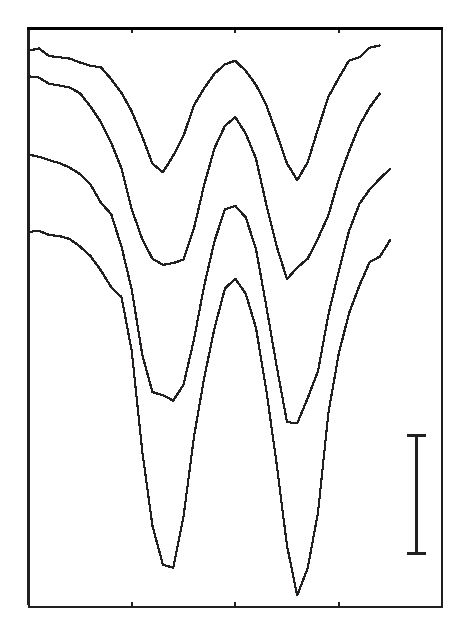
\includegraphics[width=\unitlength]{pics/picRaspredelenie.eps}}%
    \put(-0.036,-0.01){\color[rgb]{0,0,0}\makebox(0,0)[lb]{\smash{$-10$}}}%
    \put(0.212,-0.01){\color[rgb]{0,0,0}\makebox(0,0)[lb]{\smash{$-5$}}}%
    \put(0.484,-0.01){\color[rgb]{0,0,0}\makebox(0,0)[lb]{\smash{$0$}}}%
    \put(0.72,-0.01){\color[rgb]{0,0,0}\makebox(0,0)[lb]{\smash{$5$}}}%
    \put(0.944,-0.01){\color[rgb]{0,0,0}\makebox(0,0)[lb]{\smash{$10$}}}%
    \put(0.42942512,-0.07){\color[rgb]{0,0,0}\makebox(0,0)[lb]{\smash{$r$\,(см)}}}%
    \put(0.766,0.29){\color[rgb]{0,0,0}\makebox(0,0)[lb]{\smash{$4$\,мГс}}}%
    \put(0.88,1.3){\color[rgb]{0,0,0}\makebox(0,0)[lb]{\smash{$(1)$}}}%
    \put(0.88,1.2){\color[rgb]{0,0,0}\makebox(0,0)[lb]{\smash{$(2)$}}}%
    \put(0.88,1.03){\color[rgb]{0,0,0}\makebox(0,0)[lb]{\smash{$(3)$}}}%
    \put(0.88,0.86){\color[rgb]{0,0,0}\makebox(0,0)[lb]{\smash{$(4)$}}}%
  \end{picture}%
\endgroup

   \vspace{0.5cm}
   \caption{Поперечная структура диамагнитного возмущения вблизи ($z=3.5$~см) рамочной антенны при различных концентрациях фоновой плазмы $n_{e}$: $(1)$ $n_{e}=6.0\cdot{}10^{9}$~см$^{-3}$, $(2)$ $n_{e}=7.4\cdot{}10^{9}$~см$^{-3}$, $(3)$  $n_{e}=1.2\cdot{}10^{10}$~см$^{-3}$, $(4)$ $n_{e}=3.1\cdot{}10^{10}$~см$^{-3}$. Положение минимумов соответствует положению зонда напротив витков рамочной антенны.}
   \label{fig:ne_distr}
\end{figure}

Продольный масштаб диамагнитного возмущения характеризуется длиной свободного пробега электронов $l_{ei}$ и варьируется в пределах $l_{ei}\simeq{}50\div{}100$\,см, достигая, таким образом, полной длины плазменного столба. 

%\begin{figure}[H]
%    \centering
%    \includegraphics*[width=0.5\linewidth]{pic1HARM_L3+L1RAD}
%    \caption{Структура диамагнитного возмущения, регистрируемая в различных поперечных сечениях плазменного столба: $(1)\ {}\Delta{}z=3.5$\,см и $(2)\ {}\Delta{}z=41.5$\,см. Величина внешнего магнитного поля $B_{0}=25$\, Гс, концентрация плазмы $n_{e}=10^{10}$\,см$^{-3}$.}
%    \label{fig:pic1HARM_L3+L1RAD}
%\end{figure}

\subsection{Параметрическое возбуждение НЧ волн}
Как было отмечено во введении, при амплитудной модуляции ВЧ сигнала, подводимого к антенне, в плазме возбуждаются НЧ электромагнитные поля на частоте модуляции, регистрация и исследование которых было целью описываемых ниже экспериментов.
На \mbox{рис.\ref{fig:phase_composite}$a$} приведены  осциллограммы НЧ сигналов, регистрируемые при подаче на антенну импульса ВЧ накачки с несущей частотой $f\simeq{}f_{ce}$ (ЭЦР) и модулированного по амплитуде с частотой $f_{m}$; различные осциллограммы соответствуют различному радиальному удалению $r$ магнитного датчика от антенны; измерения проводились с шагом $\Delta{}r = 2$~см. Как видно из этого графика, НЧ возмущение внешнего магнитного поля распространяется поперек плазменного столба с конечной фазовой скоростью $v_{\perp}$, увеличивающейся с частотой модуляции ВЧ импульса накачки (\mbox{рис.\ref{fig:phase_composite}$b$}).
\begin{figure}[H]
  \centering
  \def\svgwidth{0.6\columnwidth} % sets the image width, this is optional
  %% Creator: Inkscape inkscape 0.48.0, www.inkscape.org
%% PDF/EPS/PS + LaTeX output extension by Johan Engelen, 2010
%% Accompanies image file 'phase_composite.eps' (pdf, eps, ps)
%%
%% To include the image in your LaTeX document, write
%%   \input{<filename>.pdf_tex}
%%  instead of
%%   \includegraphics{<filename>.pdf}
%% To scale the image, write
%%   \def\svgwidth{<desired width>}
%%   \input{<filename>.pdf_tex}
%%  instead of
%%   \includegraphics[width=<desired width>]{<filename>.pdf}
%%
%% Images with a different path to the parent latex file can
%% be accessed with the `import' package (which may need to be
%% installed) using
%%   \usepackage{import}
%% in the preamble, and then including the image with
%%   \import{<path to file>}{<filename>.pdf_tex}
%% Alternatively, one can specify
%%   \graphicspath{{<path to file>/}}
%% 
%% For more information, please see info/svg-inkscape on CTAN:
%%   http://tug.ctan.org/tex-archive/info/svg-inkscape

\begingroup
  \makeatletter
  \providecommand\color[2][]{%
    \errmessage{(Inkscape) Color is used for the text in Inkscape, but the package 'color.sty' is not loaded}
    \renewcommand\color[2][]{}%
  }
  \providecommand\transparent[1]{%
    \errmessage{(Inkscape) Transparency is used (non-zero) for the text in Inkscape, but the package 'transparent.sty' is not loaded}
    \renewcommand\transparent[1]{}%
  }
  \providecommand\rotatebox[2]{#2}
  \ifx\svgwidth\undefined
    \setlength{\unitlength}{228.42889404pt}
  \else
    \setlength{\unitlength}{\svgwidth}
  \fi
  \global\let\svgwidth\undefined
  \makeatother
  \begin{picture}(1,1.91032911)%
    \put(0,0){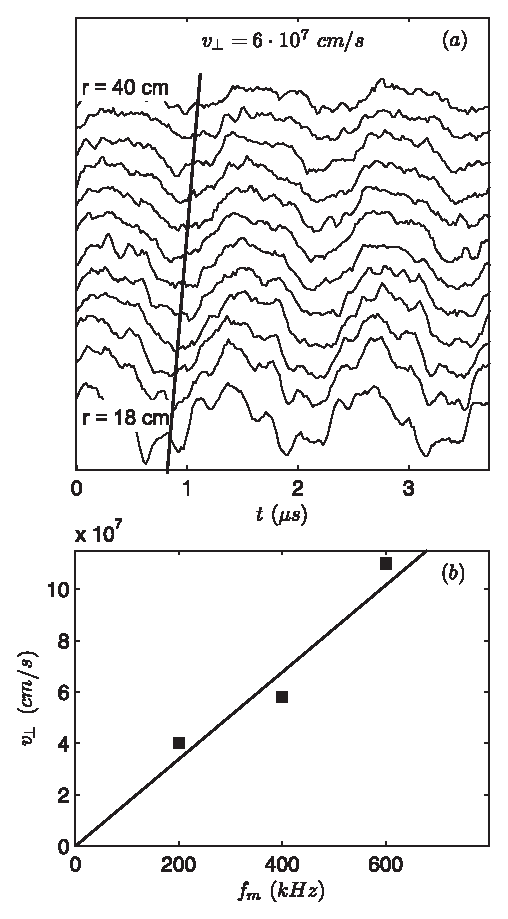
\includegraphics[width=\unitlength]{pics/phase_composite.eps}}%
    \put(0.12,0.868){\color[rgb]{0,0,0}\makebox(0,0)[lb]{\smash{$0$}}}%
    \put(0.353,0.868){\color[rgb]{0,0,0}\makebox(0,0)[lb]{\smash{$1$}}}%
    \put(0.58451047,0.868){\color[rgb]{0,0,0}\makebox(0,0)[lb]{\smash{$2$}}}%
    \put(0.81446356,0.868){\color[rgb]{0,0,0}\makebox(0,0)[lb]{\smash{$3$}}}%
    \put(0.14,1.03){\color[rgb]{0,0,0}\makebox(0,0)[lb]{\smash{$r=18$\,см}}}%
    \put(0.145,1.71){\color[rgb]{0,0,0}\makebox(0,0)[lb]{\smash\bfseries{$r=40$\,см}}}%
    \put(0.5226,0.82){\color[rgb]{0,0,0}\makebox(0,0)[lb]{\smash{$t$\,(мкс)}}}%
    \put(0.9,1.74){\color[rgb]{0,0,0}\makebox(0,0)[lb]{\smash{(a)}}}%

    \put(0.48545375,0.0){\color[rgb]{0,0,0}\makebox(0,0)[lb]{\smash{$f_m$\,(кГц)}}}%
    \put(0.11929763,0.09){\color[rgb]{0,0,0}\makebox(0,0)[lb]{\smash{$0$}}}%
    \put(0.313,0.09){\color[rgb]{0,0,0}\makebox(0,0)[lb]{\smash{$200$}}}%
    \put(0.53,0.09){\color[rgb]{0,0,0}\makebox(0,0)[lb]{\smash{$400$}}}%
    \put(0.748,0.09){\color[rgb]{0,0,0}\makebox(0,0)[lb]{\smash{$600$}}}%
    \put(0.08,0.12){\color[rgb]{0,0,0}\makebox(0,0)[lb]{\smash{$0$}}}%
    \put(0.08,0.232){\color[rgb]{0,0,0}\makebox(0,0)[lb]{\smash{$2$}}}%
    \put(0.08,0.34){\color[rgb]{0,0,0}\makebox(0,0)[lb]{\smash{$4$}}}%
    \put(0.08, 0.448){\color[rgb]{0,0,0}\makebox(0,0)[lb]{\smash{$6$}}}%
    \put(0.08,0.552){\color[rgb]{0,0,0}\makebox(0,0)[lb]{\smash{$8$}}}%
    \put(0.063,0.66){\color[rgb]{0,0,0}\makebox(0,0)[lb]{\smash{$10$}}}%
    \put(0.123,0.77){\color[rgb]{0,0,0}\makebox(0,0)[lb]{\smash{$\times{}10^7$}}}%
    \put(0.037,0.37){\color[rgb]{0,0,0}\rotatebox{90}{\makebox(0,0)[lb]{\smash{$v_\perp$\,(см/с)}}}}%
    \put(0.9,0.68){\color[rgb]{0,0,0}\makebox(0,0)[lb]{\smash{(б)}}}%
  \end{picture}%
\endgroup

  \caption{$(a)$ Осциллограммы НЧ сигналов, регистрируемые при подаче на антенну амплитудно--модулированного с частотой $f_{m}$ импульса ВЧ накачки в условиях ЭЦР, при различном радиальном удалении $r$ магнитного зонда от антенны ($f_{m} = 400$\, кГц, $f=66.5$\,МГц $\simeq f_{ce}$, $P\simeq 300$\,Вт). $(b)$ Зависимость поперечной скорости распространения $v_{\perp}$ НЧ возмущений внешнего магнитного поля от частоты модуляции $f_{m}$ импульса ВЧ накачки.}
  \label{fig:phase_composite}
\end{figure} 



\begin{figure}[H]
  \centering
  \def\svgwidth{0.6\columnwidth} % sets the image width, this is optional
  %% Creator: Inkscape inkscape 0.48.0, www.inkscape.org
%% PDF/EPS/PS + LaTeX output extension by Johan Engelen, 2010
%% Accompanies image file 'picLF2+LF4.eps' (pdf, eps, ps)
%%
%% To include the image in your LaTeX document, write
%%   \input{<filename>.pdf_tex}
%%  instead of
%%   \includegraphics{<filename>.pdf}
%% To scale the image, write
%%   \def\svgwidth{<desired width>}
%%   \input{<filename>.pdf_tex}
%%  instead of
%%   \includegraphics[width=<desired width>]{<filename>.pdf}
%%
%% Images with a different path to the parent latex file can
%% be accessed with the `import' package (which may need to be
%% installed) using
%%   \usepackage{import}
%% in the preamble, and then including the image with
%%   \import{<path to file>}{<filename>.pdf_tex}
%% Alternatively, one can specify
%%   \graphicspath{{<path to file>/}}
%% 
%% For more information, please see info/svg-inkscape on CTAN:
%%   http://tug.ctan.org/tex-archive/info/svg-inkscape

\begingroup
  \makeatletter
  \providecommand\color[2][]{%
    \errmessage{(Inkscape) Color is used for the text in Inkscape, but the package 'color.sty' is not loaded}
    \renewcommand\color[2][]{}%
  }
  \providecommand\transparent[1]{%
    \errmessage{(Inkscape) Transparency is used (non-zero) for the text in Inkscape, but the package 'transparent.sty' is not loaded}
    \renewcommand\transparent[1]{}%
  }
  \providecommand\rotatebox[2]{#2}
  \ifx\svgwidth\undefined
    \setlength{\unitlength}{207.0671875pt}
  \else
    \setlength{\unitlength}{\svgwidth}
  \fi
  \global\let\svgwidth\undefined
  \makeatother
  \begin{picture}(1,1.12792072)%
    \put(0,0){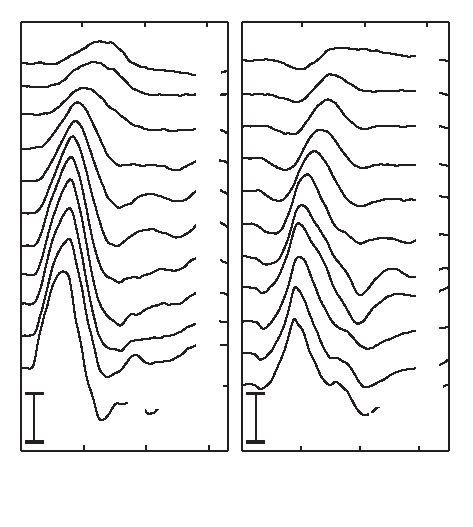
\includegraphics[width=\unitlength]{pics/picLF2+LF4.eps}}%
    \put(0,0.09){\color[rgb]{0,0,0}\makebox(0,0)[lb]{\smash{$0$}}}%
    \put(0.138,0.09){\color[rgb]{0,0,0}\makebox(0,0)[lb]{\smash{$1$}}}%
    \put(0.28,0.09){\color[rgb]{0,0,0}\makebox(0,0)[lb]{\smash{$2$}}}%
    \put(0.426,0.09){\color[rgb]{0,0,0}\makebox(0,0)[lb]{\smash{$3$}}}%
    \put(0.5,0.09){\color[rgb]{0,0,0}\makebox(0,0)[lb]{\smash{$0$}}}%
    \put(0.636,0.09){\color[rgb]{0,0,0}\makebox(0,0)[lb]{\smash{$1$}}}%
    \put(0.77,0.09){\color[rgb]{0,0,0}\makebox(0,0)[lb]{\smash{$2$}}}%
    \put(0.904,0.09){\color[rgb]{0,0,0}\makebox(0,0)[lb]{\smash{$3$}}}%
    \put(0.67,0.006){\color[rgb]{0,0,0}\makebox(0,0)[lb]{\smash{$t$\,(мкс)}}}%
    \put(0.18,0.006){\color[rgb]{0,0,0}\makebox(0,0)[lb]{\smash{$t$\,(мкс)}}}%
    \put(0.07,0.16){\color[rgb]{0,0,0}\makebox(0,0)[lb]{\smash{$0.2$\,мГc}}}%
    \put(0.02,1.06){\color[rgb]{0,0,0}\makebox(0,0)[lb]{\smash{$(а)$}}}%
    \put(0.52,1.06){\color[rgb]{0,0,0}\makebox(0,0)[lb]{\smash{$(б)$}}}%
    \put(0.41,0.98){\color[rgb]{0,0,0}\makebox(0,0)[lb]{\smash{$50$}}}%
    \put(0.41,0.93){\color[rgb]{0,0,0}\makebox(0,0)[lb]{\smash{$46$}}}%
    \put(0.41,0.85){\color[rgb]{0,0,0}\makebox(0,0)[lb]{\smash{$42$}}}%
    \put(0.41,0.78){\color[rgb]{0,0,0}\makebox(0,0)[lb]{\smash{$38$}}}%
    \put(0.41,0.716){\color[rgb]{0,0,0}\makebox(0,0)[lb]{\smash{$34$}}}%
    \put(0.41,0.64){\color[rgb]{0,0,0}\makebox(0,0)[lb]{\smash{$30$}}}%
    \put(0.41,0.56){\color[rgb]{0,0,0}\makebox(0,0)[lb]{\smash{$26$}}}%
    \put(0.41,0.48){\color[rgb]{0,0,0}\makebox(0,0)[lb]{\smash{$22$}}}%
    \put(0.41,0.412){\color[rgb]{0,0,0}\makebox(0,0)[lb]{\smash{$18$}}}%
    \put(0.41,0.35){\color[rgb]{0,0,0}\makebox(0,0)[lb]{\smash{$14$}}}%
    \put(0.27,0.24){\color[rgb]{0,0,0}\makebox(0,0)[lb]{\smash{$r=10$\,см}}}%
    \put(0.57646597,0.16){\color[rgb]{0,0,0}\makebox(0,0)[lb]{\smash{$0.2$\,мГс}}}%
    \put(0.774,0.24){\color[rgb]{0,0,0}\makebox(0,0)[lb]{\smash{$r=10$\,см}}}%
    \put(0.91,0.31){\color[rgb]{0,0,0}\makebox(0,0)[lb]{\smash{$14$}}}%
    \put(0.91,0.39){\color[rgb]{0,0,0}\makebox(0,0)[lb]{\smash{$18$}}}%
    \put(0.91,0.47){\color[rgb]{0,0,0}\makebox(0,0)[lb]{\smash{$22$}}}%
    \put(0.91,0.53){\color[rgb]{0,0,0}\makebox(0,0)[lb]{\smash{$26$}}}%
    \put(0.91,0.61){\color[rgb]{0,0,0}\makebox(0,0)[lb]{\smash{$30$}}}%
    \put(0.91,0.7){\color[rgb]{0,0,0}\makebox(0,0)[lb]{\smash{$34$}}}%
    \put(0.91,0.77){\color[rgb]{0,0,0}\makebox(0,0)[lb]{\smash{$38$}}}%
    \put(0.91,0.86){\color[rgb]{0,0,0}\makebox(0,0)[lb]{\smash{$42$}}}%
    \put(0.91,0.94){\color[rgb]{0,0,0}\makebox(0,0)[lb]{\smash{$46$}}}%
    \put(0.91,1.02){\color[rgb]{0,0,0}\makebox(0,0)[lb]{\smash{50}}}%
  \end{picture}%
\endgroup

  \caption{Осциллограммы возмущения продольной компоненты магнитного поля, регистрируемые приемным зондом , расположенным на расстояних $\Delta{}z=3.5$\,см $(a)$ и $\Delta{}z=41.5$\,см $(b)$ от излучающей рамончой  антенны, и смещенным на расстояние $r$ относительно ее оси.}
  \label{fig:picLF2+LF4}
\end{figure} 

Измерения позволяют однозначно идентифицировать НЧ поля как косые волны свистового диапазона, продольная фазовая скорость которых $v_{\parallel}\sim 10^8 \div 10^9$\,см/с (результаты не представлены) значительно превышает поперечную фазовую скорость $v_{\perp}\sim 10^7 \div 10^8$\,см/с (\mbox{рис.\ref{fig:phase_composite}$a$}). Наблюдается возбуждение волн конической рефракции (англ. Gendrin mode~\ref{Helliwell}), волновой вектор которых практически перпендикулярен к внешнему магнитному полю, а групповая скорость направлена вдоль поля. Преимущественное возбуждение волн данного типа обусловлено геометрией ``бестелесной'' антенны, которая сильно вытянута вдоль внешнего магнитного поля (что соответствует низким продольным волновым числам $k_{\parallel}$), но имеет малый поперечный размер (что соответствует высоким поперечным волновым числам $k_{\perp}$). Поперечная фазовая скорость НЧ волн пропорциональна их частоте (\mbox{рис.\ref{fig:phase_composite}$b$)}, в соответствии с законом дисперсии волн конической рефракции ($v_{\perp}\simeq c f_m/f_{pe}$). Характерные значения амплитуды переменного магнитного поля в НЧ волнах, регистрируемых на периферии плазмы ($r\sim 20\div 40$\,см), приблизительно на $2$ порядка ниже, чем в области исходного диамагнитного возмущения вблизи антенны, и составляют $|\Delta B|\sim 10^{-4}$\,Гс.

\begin{figure}[H]
  \centering
  \def\svgwidth{0.6\columnwidth} % sets the image width, this is optional
  %% Creator: Inkscape inkscape 0.48.0, www.inkscape.org
%% PDF/EPS/PS + LaTeX output extension by Johan Engelen, 2010
%% Accompanies image file 'param_vs_dir.eps' (pdf, eps, ps)
%%
%% To include the image in your LaTeX document, write
%%   \input{<filename>.pdf_tex}
%%  instead of
%%   \includegraphics{<filename>.pdf}
%% To scale the image, write
%%   \def\svgwidth{<desired width>}
%%   \input{<filename>.pdf_tex}
%%  instead of
%%   \includegraphics[width=<desired width>]{<filename>.pdf}
%%
%% Images with a different path to the parent latex file can
%% be accessed with the `import' package (which may need to be
%% installed) using
%%   \usepackage{import}
%% in the preamble, and then including the image with
%%   \import{<path to file>}{<filename>.pdf_tex}
%% Alternatively, one can specify
%%   \graphicspath{{<path to file>/}}
%% 
%% For more information, please see info/svg-inkscape on CTAN:
%%   http://tug.ctan.org/tex-archive/info/svg-inkscape

\begingroup
  \makeatletter
  \providecommand\color[2][]{%
    \errmessage{(Inkscape) Color is used for the text in Inkscape, but the package 'color.sty' is not loaded}
    \renewcommand\color[2][]{}%
  }
  \providecommand\transparent[1]{%
    \errmessage{(Inkscape) Transparency is used (non-zero) for the text in Inkscape, but the package 'transparent.sty' is not loaded}
    \renewcommand\transparent[1]{}%
  }
  \providecommand\rotatebox[2]{#2}
  \ifx\svgwidth\undefined
    \setlength{\unitlength}{230.01171875pt}
  \else
    \setlength{\unitlength}{\svgwidth}
  \fi
  \global\let\svgwidth\undefined
  \makeatother
  \begin{picture}(1,1.4490634)%
    \put(0,0){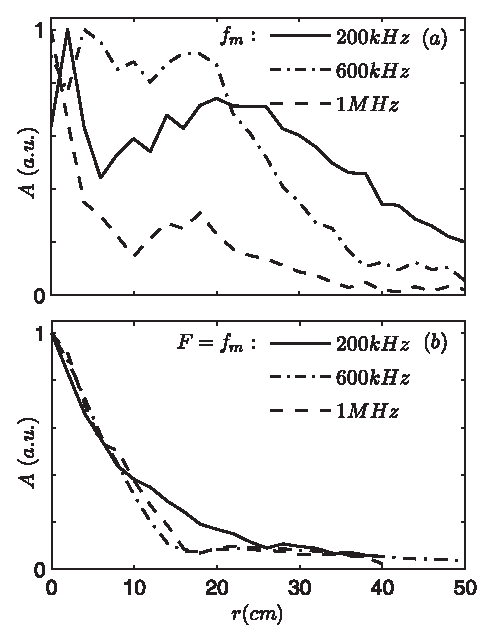
\includegraphics[width=\unitlength]{pics/param_vs_dir.eps}}%
    \put(0,-0.05){\color[rgb]{0,0,0}\makebox(0,0)[lb]{\smash{$0$}}}%
    \put(0.18,-0.05){\color[rgb]{0,0,0}\makebox(0,0)[lb]{\smash{$10$}}}%
    \put(0.372,-0.05){\color[rgb]{0,0,0}\makebox(0,0)[lb]{\smash{$20$}}}%
    \put(0.578,-0.05){\color[rgb]{0,0,0}\makebox(0,0)[lb]{\smash{$30$}}}%
    \put(0.769,-0.05){\color[rgb]{0,0,0}\makebox(0,0)[lb]{\smash{$40$}}}%
    \put(0.968,-0.05){\color[rgb]{0,0,0}\makebox(0,0)[lb]{\smash{$50$}}}%
    \put(0.44,-0.1){\color[rgb]{0,0,0}\makebox(0,0)[lb]{\smash{$r$\,(см)}}}%
    \put(0.7,0.37){\color[rgb]{0,0,0}\makebox(0,0)[lb]{\smash{$1$\,МГц}}}%
    \put(0.7,0.45){\color[rgb]{0,0,0}\makebox(0,0)[lb]{\smash{$600$\,кГц}}}%
    \put(0.7,0.53){\color[rgb]{0,0,0}\makebox(0,0)[lb]{\smash{$200$\,кГц}}}%
    \put(0.9,0.54){\color[rgb]{0,0,0}\makebox(0,0)[lb]{\smash{$(б)$}}}%
    \put(0.32,0.532){\color[rgb]{0,0,0}\makebox(0,0)[lb]{\smash{$F=f_m:$}}}%
    \put(-0.04,-0.01){\color[rgb]{0,0,0}\makebox(0,0)[lb]{\smash{$0$}}}%
    \put(-0.04,0.58){\color[rgb]{0,0,0}\makebox(0,0)[lb]{\smash{$1$}}}%
    \put(0.7,1.26){\color[rgb]{0,0,0}\makebox(0,0)[lb]{\smash{$200$\,кГц}}}%
    \put(0.7,1.186){\color[rgb]{0,0,0}\makebox(0,0)[lb]{\smash{$600$\,кГц}}}%
    \put(0.7,1.104){\color[rgb]{0,0,0}\makebox(0,0)[lb]{\smash{$1$\,МГц}}}%

    \put(0.9,1.264){\color[rgb]{0,0,0}\makebox(0,0)[lb]{\smash{$(а)$}}}%
    \put(-0.04,0.65){\color[rgb]{0,0,0}\makebox(0,0)[lb]{\smash{$0$}}}%
    \put(-0.04,1.27){\color[rgb]{0,0,0}\makebox(0,0)[lb]{\smash{$1$}}}%
    \put(-0.06,0.9){\color[rgb]{0,0,0}\rotatebox{90}{\makebox(0,0)[lb]{\smash{$A$\,(у.е.)}}}}%
    \put(-0.06,0.23){\color[rgb]{0,0,0}\rotatebox{90}{\makebox(0,0)[lb]{\smash{$A$\,(у.е.)}}}}%
    \put(0.442,1.268){\color[rgb]{0,0,0}\makebox(0,0)[lb]{\smash{$f_m$:}}}%
  \end{picture}%
\endgroup

  \vspace{0.7cm}
  \caption{$(a)$ Радиальное распределение амплитуды НЧ волн свистового диапазона, возбуждаемых амплитудно-модулированным ВЧ сигналом в условиях ЭЦР ($f=66.5$\,МГц $\simeq f_{ce}$, $P\simeq 300$\,Вт) при различных частотах модуляции $f_{m}$, и регистрируемых на расстоянии $z=48$\,см от антенны. $(b)$ Радиальное распределение амплитуды пробных НЧ волн, возбуждаемых при непосредственной подаче НЧ сигнала на рамочную антенну; измерения выполнены на тех же частотах $F=f_m$ в том же сечении $z$.}
  \label{fig:param_vs_dir}
\end{figure} 
 
Эксперименты показывают, что поперечные размеры области, занятой НЧ волнами, которые регистрируются практически по всему сечению плазменного столба (\mbox{рис.\ref{fig:param_vs_dir}$a$}), существенно превосходят диаметр силовой трубки, содержащей ускоренные электроны ($r < 10$\,см). Кроме того, ускорение электронов амплитудно-мо\-ду\-ли\-ро\-ван\-ным ВЧ полем в условиях ЭЦР позволяет возбудить НЧ волны в большей области плазмы, чем при их излучении с помощью антенны, к которой подводится НЧ сигнал. На \mbox{рис.\ref{fig:param_vs_dir}$b$} приводится радиальное распределение амплитуды пробных НЧ волн, возбуждаемых при непосредственной подаче НЧ сигнала на рамочную антенну. Видно, что в этом случае НЧ волны локализованы вблизи оси плазменного столба на поперечном масштабе $r < 20$\,см, обусловленном размерами излучателя, и не достигают периферии плазмы, как при параметрическом возбуждении амплитудно-модулированным ВЧ полем.   

Амплитуда НЧ волн, возбуждаемых при ускорении электронов ам\-пли\-ту\-дно-мо\-ду\-ли\-ро\-ван\-ным ВЧ сигналом, резонансным образом зависит от отношения несущей частоты $f$ к электронной циклотронной частоте (\mbox{рис.\ref{fig:param_vs_dir_res}}). Ширина резонанса увеличивается с повышением частоты модуляции (\mbox{рис.\ref{fig:param_vs_dir_res}$a$}), что обусловлено увеличением полной ширины частотного спектра ВЧ поля, ускоряющего электроны. Так как амплитуда НЧ волн максимальна в условиях ЭЦР, предлагаемый резонансный механизм генерации, вероятно, эффективнее других параметрических механизмов, использующих, например, пондеромоторную нелинейность плазмы~\ref{Gushchin}.
\begin{figure}[H]
  \centering
  \def\svgwidth{0.6\columnwidth} % sets the image width, this is optional
  %% Creator: Inkscape inkscape 0.48.0, www.inkscape.org
%% PDF/EPS/PS + LaTeX output extension by Johan Engelen, 2010
%% Accompanies image file 'param_vs_dir_res.eps' (pdf, eps, ps)
%%
%% To include the image in your LaTeX document, write
%%   \input{<filename>.pdf_tex}
%%  instead of
%%   \includegraphics{<filename>.pdf}
%% To scale the image, write
%%   \def\svgwidth{<desired width>}
%%   \input{<filename>.pdf_tex}
%%  instead of
%%   \includegraphics[width=<desired width>]{<filename>.pdf}
%%
%% Images with a different path to the parent latex file can
%% be accessed with the `import' package (which may need to be
%% installed) using
%%   \usepackage{import}
%% in the preamble, and then including the image with
%%   \import{<path to file>}{<filename>.pdf_tex}
%% Alternatively, one can specify
%%   \graphicspath{{<path to file>/}}
%% 
%% For more information, please see info/svg-inkscape on CTAN:
%%   http://tug.ctan.org/tex-archive/info/svg-inkscape

\begingroup
  \makeatletter
  \providecommand\color[2][]{%
    \errmessage{(Inkscape) Color is used for the text in Inkscape, but the package 'color.sty' is not loaded}
    \renewcommand\color[2][]{}%
  }
  \providecommand\transparent[1]{%
    \errmessage{(Inkscape) Transparency is used (non-zero) for the text in Inkscape, but the package 'transparent.sty' is not loaded}
    \renewcommand\transparent[1]{}%
  }
  \providecommand\rotatebox[2]{#2}
  \ifx\svgwidth\undefined
    \setlength{\unitlength}{224.4984375pt}
  \else
    \setlength{\unitlength}{\svgwidth}
  \fi
  \global\let\svgwidth\undefined
  \makeatother
  \begin{picture}(1,1.89401722)%
    \put(0,0){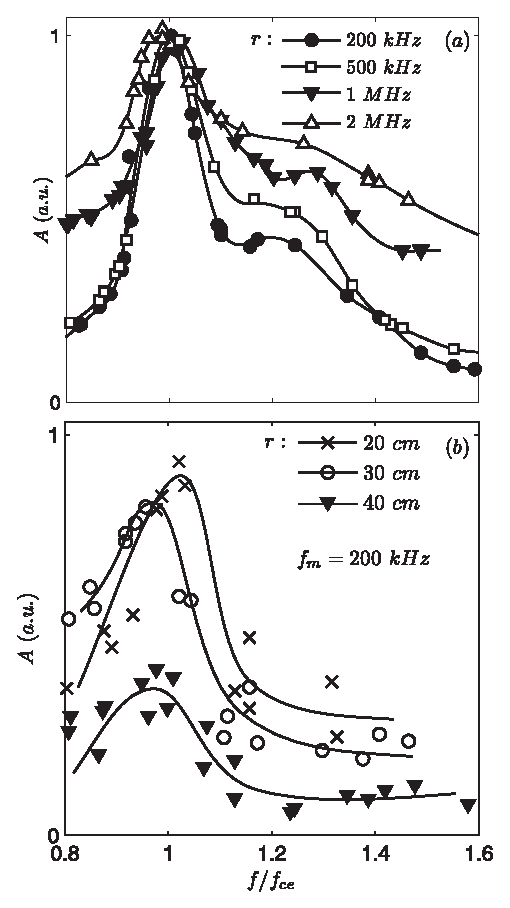
\includegraphics[width=\unitlength]{pics/param_vs_dir_res.eps}}%
    \put(0.06,1.73){\color[rgb]{0,0,0}\makebox(0,0)[lb]{\smash{$1$}}}%
    \put(0.06,0.97){\color[rgb]{0,0,0}\makebox(0,0)[lb]{\smash{$0$}}}%
    \put(0.06,0.05){\color[rgb]{0,0,0}\makebox(0,0)[lb]{\smash{$0$}}}%
    \put(0.06,0.89){\color[rgb]{0,0,0}\makebox(0,0)[lb]{\smash{$1$}}}%
    \put(0.0687818,0.01){\color[rgb]{0,0,0}\makebox(0,0)[lb]{\smash{$0.8$}}}%
    \put(0.308,0.01){\color[rgb]{0,0,0}\makebox(0,0)[lb]{\smash{$1$}}}%
    \put(0.504,0.01){\color[rgb]{0,0,0}\makebox(0,0)[lb]{\smash{$1.2$}}}%
    \put(0.724,0.01){\color[rgb]{0,0,0}\makebox(0,0)[lb]{\smash{$1.4$}}}%
    \put(0.95,0.01){\color[rgb]{0,0,0}\makebox(0,0)[lb]{\smash{$1.6$}}}%
    \put(0.46547512,-0.06){\color[rgb]{0,0,0}\makebox(0,0)[lb]{\smash{$f/f_{ce}$}}}%
    \put(0.58,0.65){\color[rgb]{0,0,0}\makebox(0,0)[lb]{\smash{$f_m=200$\,кГц}}}%

    \put(0.75,0.748){\color[rgb]{0,0,0}\makebox(0,0)[lb]{\smash{$40$\,см}}}%
    \put(0.75,0.812){\color[rgb]{0,0,0}\makebox(0,0)[lb]{\smash{$30$\,см}}}%
    \put(0.75,0.874){\color[rgb]{0,0,0}\makebox(0,0)[lb]{\smash{$20$\,см}}}%
    \put(0.51,0.874){\color[rgb]{0,0,0}\makebox(0,0)[lb]{\smash{$r:$}}}%
    \put(0.5,1.723){\color[rgb]{0,0,0}\makebox(0,0)[lb]{\smash{$r:$}}}%   
    \put(0.03,0.45){\color[rgb]{0,0,0}\rotatebox{90}{\makebox(0,0)[lb]{\smash{$A$\,(у.е.)}}}}%
    \put(0.03,1.3){\color[rgb]{0,0,0}\rotatebox{90}{\makebox(0,0)[lb]{\smash{$A$\,(у.е.)}}}}%
    \put(0.88,0.88){\color[rgb]{0,0,0}\makebox(0,0)[lb]{\smash{$(б)$}}}%
    \put(0.88,1.72){\color[rgb]{0,0,0}\makebox(0,0)[lb]{\smash{$(а)$}}}%
    \put(0.713,1.548){\color[rgb]{0,0,0}\makebox(0,0)[lb]{\smash{$2$\,МГц}}}%
    \put(0.713,1.6152){\color[rgb]{0,0,0}\makebox(0,0)[lb]{\smash{$1$\,МГц}}}%
    \put(0.713,1.668){\color[rgb]{0,0,0}\makebox(0,0)[lb]{\smash{$500$\,кГц}}}%
    \put(0.713,1.72){\color[rgb]{0,0,0}\makebox(0,0)[lb]{\smash{$200$\,кГц}}}%
  \end{picture}%
\endgroup

  \vspace{0.3cm}
  \caption{$(a)$ Амплитуда НЧ волн свистового диапазона на частотах $F=f_m$, возбуждаемых амплитудно-модулированным ВЧ сигналом ($f=66.5$\,МГц, $P=300$\,Вт), в зависимости от отношения $f/f_{ce}$; измерения выполнены на расстоянии $z=64$\,см от антенны вблизи оси плазменного столба $r=0$\,см. $(b)$ Амплитуда НЧ волн свистового диапазона на частоте $f=f_m=200$\,кГц, возбуждаемых амплитудно-модулированным ВЧ сигналом, в зависимости от отношения $f/f_{ce}$ в сечении $z=64$\,см при различных радиальных позициях $r$ измерительного зонда.}
  \label{fig:param_vs_dir_res}
\end{figure}

Подавая на излучающую антенну сигнал ВЧ накачки, апмлитудно--мо\-ду\-ли\-ро\-ван\-ного меандром с чатотой повтороения $f_m=200\,kHz$ в условиях ЭЦР (\mbox{рис.\ref{fig:h_sep_base}}), можно наблюдать изменение спектра сигнала, принимаемого на различном радиальном удалении $r$ от излучающей антенны (\mbox{рис.\ref{fig:h_sep}}).
\begin{figure}[H]
    \centering
    \includegraphics*[width=0.8\columnwidth]{pics/h_separation_base}
    \caption{Спектр огибающей сигнала ВЧ накачки, подаваемого на рамочную антенну}
    \label{fig:h_sep_base}
 \end{figure}

%\begin{figure}[H]
%    \centering
%    \psfrag{200}{200}
%    \includegraphics*[width=0.8\columnwidth]{combine.eps}
%   
%    \label{fig:h_sep}
%\end{figure}
\begin{figure}
   \centering
   \def\svgwidth{0.7\columnwidth} % sets the image width, this is optional
   %% Creator: Inkscape inkscape 0.48pre0, www.inkscape.org
%% PDF/EPS/PS + LaTeX output extension by Johan Engelen, 2010
%% Accompanies image file 'h_separation' (pdf, eps, ps)
%%
%% To include the image in your LaTeX document, write
%%   \input{<filename>.tex}
%%  instead of
%%   \includegraphics{<filename>.pdf}
%% To scale the image, write
%%   \def{\svgwidth}{<desired width>}
%%   \input{<filename>.tex}
%%  instead of
%%   \includegraphics[width=<desired width>]{<filename>.pdf}

\begingroup
  \makeatletter
  \providecommand\color[2][]{%
    \errmessage{(Inkscape) Color is used for the text in Inkscape, but the package 'color.sty' is not loaded}
    \renewcommand\color[2][]{}%
  }
  \providecommand\transparent[1]{%
    \errmessage{(Inkscape) Transparency is used (non-zero) for the text in Inkscape, but the package 'transparent.sty' is not loaded}
    \renewcommand\transparent[1]{}%
  }
  \providecommand\rotatebox[2]{#2}
  \ifx\svgwidth\undefined
    \setlength{\unitlength}{335pt}
  \else
    \setlength{\unitlength}{\svgwidth}
  \fi
  %\setlength{\baseline}{0.04}
  \global\let\svgwidth\undefined
  \makeatother
  \begin{picture}(1,1.61179619)%
    \put(0,0){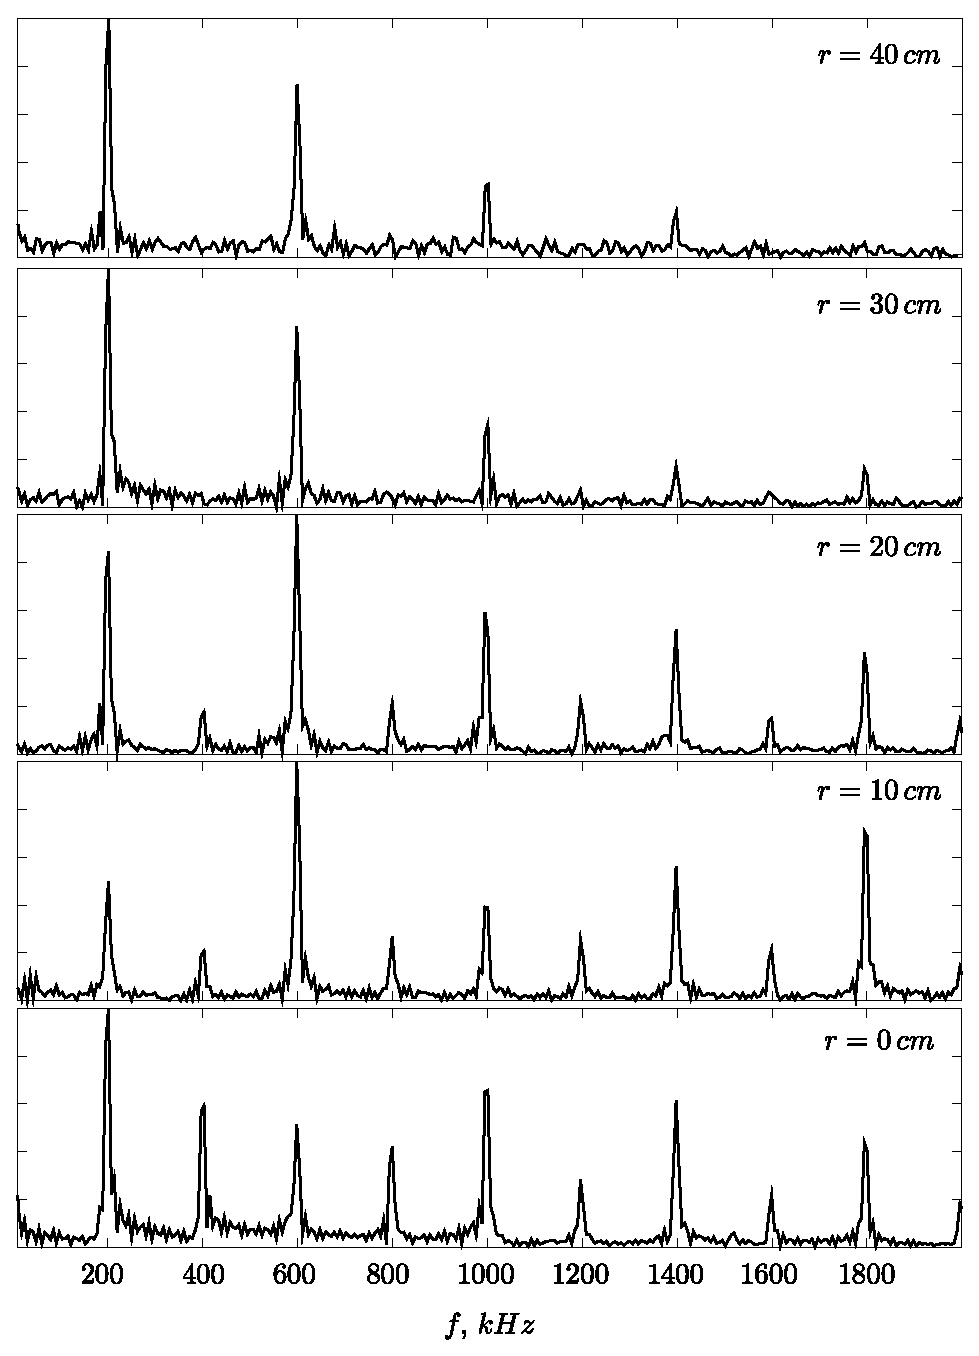
\includegraphics[width=\unitlength]{pics/h_separation.eps}}%
    \put(0.07,-0.04459907){\makebox(0,0)[lb]{\smash{$200$}}}%
    \put(0.168,-0.04459907){\makebox(0,0)[lb]{\smash{$400$}}}%
    \put(0.266,-0.04459907){\makebox(0,0)[lb]{\smash{$600$}}}%
    \put(0.368,-0.04459907){\makebox(0,0)[lb]{\smash{$800$}}}%
    \put(0.458,-0.04459907){\makebox(0,0)[lb]{\smash{$1000$}}}%
    \put(0.556,-0.04459907){\makebox(0,0)[lb]{\smash{$1200$}}}%
    \put(0.654,-0.04459907){\makebox(0,0)[lb]{\smash{$1400$}}}%
    \put(0.756,-0.04459907){\makebox(0,0)[lb]{\smash{$1600$}}}%
    \put(0.854,-0.04459907){\makebox(0,0)[lb]{\smash{$1800$}}}%
    \put(0.436,-0.12){\makebox(0,0)[lb]{\smash{$f$\,(кГц)}}}%
    \put(-0.1,-0.005 ){\makebox(0,0)[lb]{\smash{$-40$}}}%
    \put(-0.1,0.07){\makebox(0,0)[lb]{\smash{$-30$}}}%
    \put(-0.1,0.15){\makebox(0,0)[lb]{\smash{$-20$}}}%
    \put(-0.1,0.227){\makebox(0,0)[lb]{\smash{$-10$}}}%
    \put(-0.05,0.3){\makebox(0,0)[lb]{\smash{$0$}}}%
    \put(-0.15,0.78){\rotatebox{90}{\makebox(0,0)[lb]{\smash{$A$\,(дБ)}}}}%

    \put(0.8,0.27){\makebox(0,0)[lb]{\smash{$r=0$\,cм}}}%

    \put(-0.1,0.41){\makebox(0,0)[lb]{\smash{$-30$}}}%
    \put(-0.1,0.488){\makebox(0,0)[lb]{\smash{$-20$}}}%
    \put(-0.1,0.565){\makebox(0,0)[lb]{\smash{$-10$}}}%
    \put(-0.05,0.638){\makebox(0,0)[lb]{\smash{$0$}}}%

    \put(0.8,0.60){\makebox(0,0)[lb]{\smash{$r=10$\,см}}}%
    \put(-0.1,0.745){\makebox(0,0)[lb]{\smash{$-30$}}}%
    \put(-0.1,0.825){\makebox(0,0)[lb]{\smash{$-20$}}}%
    \put(-0.1,0.905){\makebox(0,0)[lb]{\smash{$-10$}}}%
    \put(-0.05,0.975){\makebox(0,0)[lb]{\smash{$0$}}}%
   
    \put(0.8,0.94){\makebox(0,0)[lb]{\smash{$r=20$\,см}}}%
    \put(-0.1,1.085){\makebox(0,0)[lb]{\smash{$-30$}}}%
    \put(-0.1,1.165){\makebox(0,0)[lb]{\smash{$-20$}}}%
    \put(-0.1,1.242){\makebox(0,0)[lb]{\smash{$-10$}}}%
    \put(-0.05,1.315){\makebox(0,0)[lb]{\smash{$0$}}}%
   
    \put(0.8,1.28){\makebox(0,0)[lb]{\smash{$r=30$\,см}}}%
    \put(-0.1,1.42){\makebox(0,0)[lb]{\smash{$-30$}}}%
    \put(-0.1,1.5){\makebox(0,0)[lb]{\smash{$-20$}}}%
    \put(-0.1,1.584){\makebox(0,0)[lb]{\smash{$-10$}}}%
    \put(-0.05,1.655){\makebox(0,0)[lb]{\smash{$0$}}}%
   
    \put(0.8,1.615){\makebox(0,0)[lb]{\smash{$r=40$\,см}}}%
  \end{picture}%
\endgroup

   \vspace{1.0cm}
   \caption{Пространственная динамика спектра принимаемого сигнала, возбужденного импульсом ВЧ накачки ($P=300$\,Вт),  амплитудно-мо\-ду\-ли\-ро\-ван\-ным меандром с частотой повторения $f_m=200 kHz$, наблюдаемая при различном радиальном удалении от передаюшей антенны $r$ на расстоянии $z=3.5$\,cм от нее, в условиях ЭЦР ($B_0 = 25$\,Гс).}
\end{figure}

Как видно из сравнения данных, приведенных на рисунках (\mbox{рис.\ref{fig:h_sep_base}}) и (\mbox{рис.\ref{fig:h_sep}}), вблизи антенны накачки наблюдается обогащение спектра принимаемого сигнала, которое объясняется следующим образом. При негармонической модуляции импульса ВЧ накачки в условиях ЭЦР, поперечную скорость электронов $v_\perp$ после прохождения ими области, занятой ВЧ полем, в нулевом приближении, можно представить как $v_\perp=\mathfrak{Re}\sum_{n} v_{f_n}\exp(-i2\pi{}f_nt)$, где $v_{f_n}$ --- комплексная амлитуда гармоники поперечной скорости на частоте $f_n$; спектр $\{f_n\}$ соответствует огибающей сигнала ВЧ накачки. Диамагнитное возмущение $\Delta{}B$, наблюдаемое в плазме, является функцией увеличения среднего магнитного момента электронов по отношению к его фоновому значению, $\Delta{}B=\Delta\left<\mu\right>\sim{}\Delta{}\left<v_\perp^2\right>$; подставляя сюда выражение для $v_\perp$, можно получить, что спектр региструемого диамагнитного возмущения должен содержать, помимо частот $\{f_n\}$, также и комбинационные частоты $\{f_n\pm{}f_k\}$, что и подтверждается экспериментально. Однако, на достаточном удалением от антенны, в спектре принимаемого сигнала остаются только те гармоники частоты модуляции $f_m=200$\,кГц, которые присутствовали в сигнале ВЧ накачки, что, в одночастичном приближении, объясняется тем, что в плазме формуриются только те ``бестелесные'' антенны, которые соответсвуют модуляции поперечной скорости электронов с частотами из спектра  $\{f_n\}$ огибающей сигнала ВЧ накачки.
\subsection{Обсуждение результатов}
Обсудим результаты экспериментов, проведенных в данной работе. Очевидно, что при максимальной ВЧ мощности ($P\simeq300$\,Вт), подводимой к антенне, возможны сильные возмущения концентрации электронов $n_e$, обусловленные развитием различных нелинейных процессов, поскольку напряженность электрических ВЧ полей в ближней зоне достигает $E\sim 10$\,В/см, а плотность энергии ВЧ поля превышает плотность энергии теплового движения частиц плазмы. В то же время, характерное время перераспределения концентрации плазмы со звуковой скоростью на масштабах ближней зоны антенны составляет $L/v_s >20$\,мкс, превышая, в частности, период амплитудной модуляции ВЧ поля в экспериментах по параметрической генерации НЧ волн. Отсутствие заметных возмущений концентрации плазмы на указанных временах подтверждается прецизионными измерениями, выполненными зондом с СВЧ-резонатором по методике, описанной в~\ref{Yanin}. В результате, регистрируемый в возмущенной области плазмы диамагнитный эффект связан исключительно с изменением средней поперечной энергии $T_{\perp}$ электронов относительно невозмущенного значения $T_{e0}$. При типичных параметрах эксперимента ($|\Delta B|\simeq 10^{-2}$\,Гс, $n_e\simeq 10^{10}$\,см$^{-3}$, $T_{e0}\simeq 1$\,эВ) $T_{\perp}/T_{e0} \simeq 1 + B|\Delta B|/(4\pi n_{e}T_{e0}) \simeq 2.2$, т.е. поперечная энергия электронов увеличивается более чем в два раза.

Поперечная струтктура возмущений продольной компоненты магнитного поля в условиях ЭЦР воспроизводит структуру компоненты $E_{\perp}$ электрического поля в ближней зоне антенны, однако, стоит отметить, что при резонансе на второй гармонике электронной циклотронной частоты $f_{ce}$ эффективный размер рамочной антенны накачки увеличился, что связано, по-видимому, с модификацией ближнего поля антенны в присутствии плазмы.

Отдельного обсуждения заслуживает поперечная структура НЧ волн, возбуждаемых модулированным диамагнитным током и непосредственно рамочной антенной (\mbox{рис.\ref{fig:param_vs_dir}}). Эксперименты показывают, что при прямой подаче НЧ напряжения на рамочную антенну распределение амплитуды НЧ волн, возбуждаемых в плазме, имеет меньший поперечный масштаб, чем при их параметрической генерации амплитудно-модулированным ВЧ сигналом, подводимым к той же антенне. Поперечные размеры источников НЧ волн в обоих случаях одинаковы, но существенно отличаются продольные масштабы: ``бестелесная'' антенна, формируемая модулированным диамагнитным током, имеет конфигурацию соленоида, сильно вытянутого вдоль внешнего магнитного поля. При этом пространственный спектр модулированного диамагнитного тока оказывается не таким широким, как у тока в проводе одновитковой рамочной антенны. В результате, возбуждаются НЧ волны с более узким спектром волновых векторов, и пространственная структура НЧ излучения оказывается в целом шире, чем при использовании рамочной антенны.

Для интерпретации результатов измерений  НЧ полей, возбуждаемых амплитудно-модулированной ВЧ накачкой, важно, что длины волн НЧ излучения в условиях эксперимента сравнимы с размерами плазменного столба, и составляют $50\div 200$\,см. Таким образом, измерения выполняются в ближней зоне и зоне Френеля ``бестелесной'' антенны, характеризуемой сложной пространственной структурой тока ускоренных частиц. Указанным обстоятельством объясняется немонотонное изменение амплитуды НЧ полей по радиусу плазмы при $r<25$\,см (\mbox{рис.\ref{fig:param_vs_dir}$a$}). Кроме того, из \mbox{рис.\ref{fig:param_vs_dir}$a$} видно, что поперечный размер области плазмы, занятой НЧ излучением, увеличивается при понижении частоты модуляции $f_m$. Этот эффект, по-видимому, связан с изменением геометрических размеров ``бестелесной'' антенны. В частности, ее продольный масштаб определяется длиной, на которой модуляция диамагнитного тока исчезает из-за теплового разброса продольных скоростей электронов, и по порядку величины может быть оценен как $L_{eff}\sim v_{Te}/f_m$. Соответственно, с понижением частоты модуляции $f_m$ увеличивается эффективная длина излучающей области плазмы. Геометрия ``бестелесной'' антенны становится ближе к цилиндрической, и амплитуда НЧ волн медленнее убывает по радиусу плазменного столба, что и наблюдается в эксперименте.

Используя преобразования подобия, по результатам лабораторных экспериментов оценим уровень квазистационарных и НЧ возмущений магнитного поля $|\Delta B_{space}|$, которые могут быть получены в активных экспериментах в верхней ионосфере с использованием мощных антенных систем, установленных на борту КА. При мощности передатчика $P\sim100\div1000$\,Вт, нагруженного на антенну с характерными размерами $L\sim10\div100$\,м, используя значение масштабного множителя $\gamma\sim 100$, величину квазистационарных диамагнитных возмущений в силовой трубке, опирающейся на антенну, можно оценить как $|\Delta{}B_{space}|=\gamma{}^{-1}|\Delta{}B|\sim 10^{-4}\div 10^{-3}$\,Гс ($10\div100$\,нТл), что сравнимо с возмущениями магнитного поля при инжекции сильноточных ($I\sim 0.1$\,А) пучков энергичных ($W\sim 10$\,кэВ) электронов с борта КА~\ref{Orajevskiy}. Амплитуда переменного магнитного поля в ОНЧ свистовых волнах с частотами $f_{space}=\gamma{}^{-1} f_m\sim 1\div 10$\,кГц, возбуждаемых при подаче на бортовую антенну КА мощного амплитудно-модулированного сигнала, может достигать $|\Delta{}B_{space}|\sim 10^{-6}\div 10^{-5}$\,Гс ($0.1\div 1$\,нТл).  

Таким образом, результаты первых модельных экспериментов показывают, что эффект циклотронного ускорения электронов в ближней зоне антенн космического базирования может быть использован в целях генерации квазистационарных и НЧ возмущений ионосферной плазмы. Предложена схема параметрической генерации НЧ волн, основанная на ускорении электронов плазмы, окружающей КА, амплитудно-мо\-ду\-ли\-ро\-ван\-ным ВЧ сигналом в условиях ЭЦР. НЧ волны, возбуждаемые при модуляции потока ускоренных электронов в силовой трубке, опирающейся на антенну, занимают существенно большую область плазмы, чем в случае их прямого возбуждения с помощью той же антенны. Несмотря на относительную малость диамагнитных возмущений ($|\Delta{}B|/B < 10^{-3}$), повышение эффективности генерации НЧ волн достигается за счет увеличения геометрических размеров источника --- ``бестелесной'' антенны, формируемой модулированными диамагнитными токами. К достоинствам предлагаемой схемы генерации НЧ волн относится возможность широкополосной перестройки по низкой частоте. Отметим, что протяженная ``бестелесная'' антенна является антенной магнитного типа, поскольку формируется замкнутыми электронными токами, возбуждение которых не связано с модуляцией плотности плазмы. В результате реализуются предпочтительные условия для возбуждения электромагнитных НЧ волн, например --- свистовых или альфвеновских.
\clearpage
\begin{theotherbib1}
\item P.M.E.~Decreau, P.~Fergeau, V.~Krasnoselskikh et al., Ann.~Geophys. {\bf 19}, 1241 (2001).\label{WHISPER}

\item F.K.~Shuiskaya, Yu.I.~Galperin, A.A.~Serov et al., Planet.~Sp.~Sci. {\bf 38}, 173 (1990).\label{Galperin}

\item C.Y.~Huang, W.J.~Burke, D.A.~Hardy et al., J.~Geophys.~Res. {\bf 106}, 1835 (2001).\label{Huang}
\item Пулинец C.A, В.В. Селегеи, Космические исследования {\bf 23}, 113 (1985).\label{Pulinets}

\item C.J.~Rodger,  J.~Lichtenberger, G.~McDowell \& N.R.~Thomson, Radio Science, {\bf 44} (2009)\label{AWD}

\item Burch, J.~L., Space Science Reviews, {\bf 91}, 1 (2000)\label{IMAGE}

\item R.A.~Helliwell, "VLF wave stimulation experiments in the magnetosphere from Siple Station, Antarctica," Rev. of Geophysics, {\bf 26}, 551, (1988).\label{SPBEACON}

\item M.~Platino, U.S.~Inan, T.F.~Bell et al., Ann.~Geophys. {\bf 22}, 2643 (2004).\label{HAARP}

\item T.R.~Robinson, Physics Reports, {\bf 179}, 79 (1989)\label{EISCAT}

\item U.S.~Inan, T.F.~Bell, J.~Bortnik et al., J.~Geophys.~Res. {\bf 108}, 1186 (2003).\label{InanBellBortnik}

\item Rory~J.~Gamble, Craig~J.~Rodger, Mark~A.~Clivered et al., J.~Geophys.~Res. {\bf 113} A10211 (2008).\label{Rory}

\item A.G.~Demekhov, V.Y.~Trakhtengerts, M.M.~Mogilevsky, and L.M.~Zelenyi, Adv.~Sp.~Res. {\bf 32}, 355 (2003).\label{Demekhov}

\item H.G.~James, J.~Geophys.~Res. {\bf 88}, 4027, (1983).\label{James}

\item М.Е.~Гущин, С.В.~Коробков, А.В.~Костров, А.В.~Стриковский, Письма в ЖЭТФ {\bf 88}, 834 (2008).\label{Gushchin}

\item R.L.~Stenzel, Rev.~.~Instrum. {\bf 47}, 603 (1976).\label{Stenzel}

\item Д.В.~Янин, А.В.~Костров, А.И.~Смирнов, А.В.~Стриковский, ЖТФ {\bf 78}, 133 (2008).\label{Yanin}

\item И.~Г.~Кондратьев, А.~В.~Костров, А.~И.~Смирнов, А.~В.~Стриковский, А.~В.~Шашурин Зонд с СВЧ-резонаторм на отрезке двухпроводной линии. \newblock Институт прикладной физики РАН, 2001\label{UHF_probe}

\item Г.~Альвен, К.-Г.~Фельтхаммар, Космическая электродинамика \newblock М.,Мир, 1967. 260~c.\label{Alfven}

\item R.A.~Helliwell, Geophys.~Res.~Lett. {\bf 22}, 2095 (1995).\label{Helliwell}

\item S.F.~Fung, R.F.~Benson, J.L.~Green et al., Adv.~Space~Res. {\bf 30}, 2259 (2002).\label{RPI}

\item P.~Kulkarni, U.S.~Inan, T.F.~Bell, J.~Geophys.~Res. {\bf 113}, A09203 (2008).\label{Kulkarni}

\item В.Н.~Ораевский, Я.П.~Соболев, Л.Н.~Жузгов и др., Физика плазмы {\bf 27}, 343 (2001). \label{Orajevskiy}
\end{theotherbib1}
\end{document}
